
\chapter{Evaluation}
\label{chapter:Evaluation}

\section{Evaluation of static FreSh}

\noindent{\bf Setup.}
% 
We used a machine equipped with 2 Intel  Xeon E5-2650 v4 2.2GHz
CPUs with 12 cores each, and 30MB L3 cache. The machine runs
Ubuntu Linux 16.04.7. LTS and has 256GB of RAM. Code is written in C and
compiled using gcc v11.2.1 with O2 optimizations.

\noindent{\bf Datasets.}
We evaluated \Fresh\ and the competing algorithms (all algorithms are in-memory) using both real and synthetic datasets.
The synthetic data series, \emph{Random}, are generated as random-walks (i.e., cumulative sums) of 
steps that follow a Gaussian distribution (0,1).
This type of data has been extensively used
~\cite{conf/sigmod/Faloutsos1994,isax2plus,conf/kdd/Zoumpatianos2015,DBLP:journals/vldb/ZoumpatianosLIP18,DBLP:journals/pvldb/EchihabiZPB18,DBLP:journals/pvldb/EchihabiZPB19}, 
and models the distribution of stock market prices~\cite{conf/sigmod/Faloutsos1994}.
Our real datasets come from the domains of seismology and astronomy.
The seismic dataset, \emph{Seismic}, was obtained from the IRIS Seismic Data Access
archive~\cite{url/data/seismic}. It contains seismic instrument recordings from
thousands of stations worldwide and consists of 100 million data series of size 256,
i.e. its size is 100GB. 
The astronomy dataset, \emph{Astro}, represents celestial objects and was obtained 
from~\cite{journal/aa/soldi2014}. The dataset consists of 270 million data series of
size 256, i.e. its size is 265GB.
% 
Since the main memory of our machine is limited to 256GB, we only use the first 200GB
of the Astro dataset in our experiments.

\begin{table}[htbp]
    \centering
    \renewcommand{\arraystretch}{1.2} % Adjust row height for better readability
    \begin{tabular}{||c | c | c | c | c||} 
        \hline
        \textbf{Dataset} & \textbf{Data} & \textbf{Length} & \textbf{Size} & \textbf{Description}  \\ 
        & \textbf{Series} & \textbf{(floats)} & \textbf{(GB)} & \\ [0.5ex]
        \hline\hline
        Seismic & 100M & 256 & 100 & seismic records  \\ 
        \hline
        Astro & 270M & 256 & 265 & astronomical data \\ 
        \hline
        Random & 100M & 256 & 100 & random walks  \\ 
        \hline
    \end{tabular}
    \caption{Details of datasets used in experiments.}
    \label{table:datasets}
\end{table}
\clearpage
\noindent{\bf Evaluation Measures.}
% 
We measure (i) the {\em summarization time} required to calculate
the iSAX summaries and fill-in the summarization buffers, 
(ii) the {\em tree time} required to insert the items of the receive buffers in the
tree-index and (iii) the {\em query answering time} required to answer 100 queries
that are not part of the dataset. 
The  sum of the above times constitute the {\em total time}.
Experiments are repeated $5$ times and averages are reported.
All algorithms return exact results.

\subsection{Results}

\noindent{\bf \Fresh\ vs \MESSI.}
We compare \Fresh\ against \MESSI, which is the state-of-the-art blocking
in-memory data series index.To enable a fair comparison, we use an 
optimized version of the original \MESSI\ implementation,
where we have applied all the code enhancements incorporated by \Fresh.
% 
We also compare \Fresh\ against an extended version of MESSI, called \MESSIenh
, that allows several threads to concurrently populate the same sub-tree, during tree creation
(instead of using a single thread for each subtree).
This is implemented using fine-grained locks that are attached on each leaf node of a subtree.
\MESSIenh\ allows to compare the lock-free index creation phase of \Fresh\ against a more
efficient blocking one than that of original \MESSI.

Figure~\ref{fig:eval:fresh-messi-threads:random} shows that all algorithms
(\Fresh, \MESSI, and \MESSIenh) continue scaling as the number of threads is increasing,
for Seismic 100GB. This is true for all three phases. 
Moreover, the total execution time of \Fresh\ 
(Figure~\ref{fig:eval:fresh-messi-threads:random:total-from-4})
is almost the same as the total execution time of all its competitors, although it is the
only lock-free approach. 
As expected, the tree index creation time of \Fresh\ is smaller than \MESSI's 
(Figure~\ref{fig:eval:fresh-messi-threads:random:tree-from-4}), since \Fresh\ allows
subtrees to be populated concurrently by multiple threads, allowing parallelism during
this phase, in contrast to \MESSI. 
Interestingly, \Fresh\ achieves better performance than \MESSIenh, in most cases.
The results for Seismic are similar and are omitted for brevity.
Considering scalability as the size of the dataset increases, 
Figure~\ref{fig:eval:scale-dataset:random} demonstrates that \Fresh\ scales well
on all three datasets. In most cases, \Fresh\ is faster than \MESSI.
Following previous works~\cite{DBLP:journals/vldb/ZoumpatianosLIP18,PFP21-I},
we also conducted experiments with query workloads of increasing difficulty.
For these workloads, we select series at random from the collection, add to each point
Gaussian noise ($\mu = 0$, $sigma = 0.01-0.1$), and use these as our queries. 
Figure~\ref{fig:eval:scale-query-difficulty:seismic:total} presents the results for
the Seismic dataset, where \Fresh\ performs better than \MESSI\ in most cases.


%%%%%%%%%%%%%%%%%%%%%%%%% Threds Scalability FreSh-MESSI-MESSIenh RANDOM%%%%%%%%%%%%%%%%%%%%%%%%%%
\begin{figure}[htbp]
    \centering
    \begin{subfigure}{0.45\textwidth}
        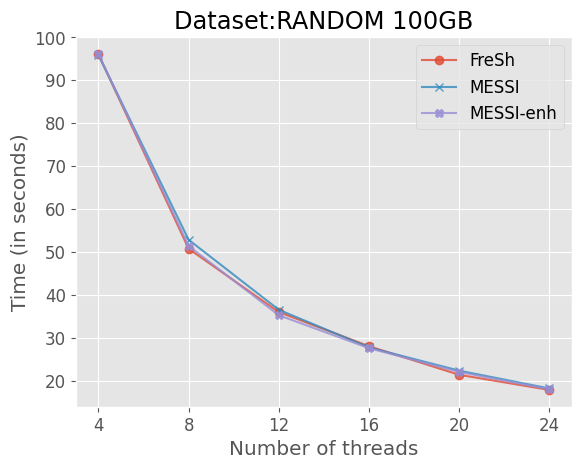
\includegraphics[width=\textwidth]{figures/Experiments/fresh-messi-threads-random-total}
        \caption{Total}
        \label{fig:eval:fresh-messi-threads:random:total-from-4}
    \end{subfigure}    
    \begin{subfigure}{0.45\textwidth}
        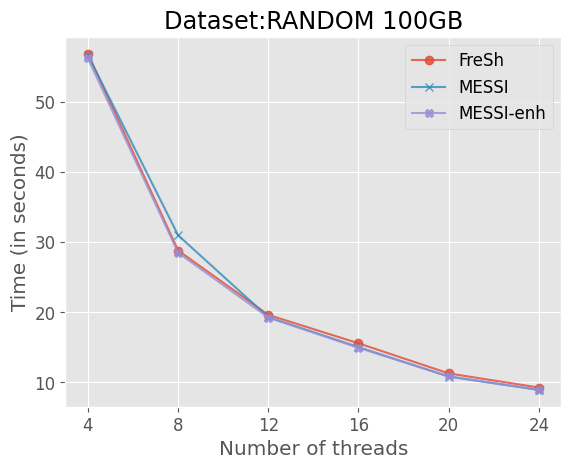
\includegraphics[width=\textwidth]{figures/Experiments/fresh-messi-threads-random-summarization}
        \caption{Summarization}
        \label{fig:eval:fresh-messi-threads:random:recbuf-from-4}
    \end{subfigure}    

    \vspace{0.2cm} % Space between rows

    \begin{subfigure}{0.45\textwidth}
        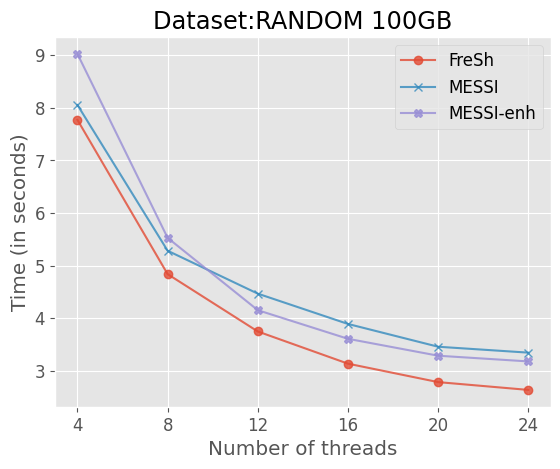
\includegraphics[width=\textwidth]{figures/Experiments/fresh-messi-threads-random-tree}
        \caption{Tree index}
        \label{fig:eval:fresh-messi-threads:random:tree-from-4}
    \end{subfigure}    
    \begin{subfigure}{0.45\textwidth}
        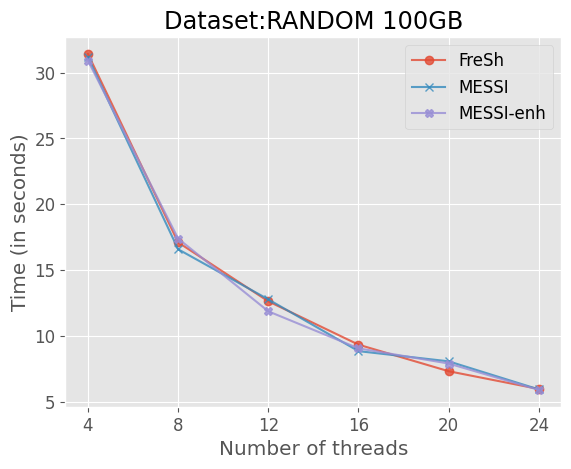
\includegraphics[width=\textwidth]{figures/Experiments/fresh-messi-threads-random-query}
        \caption{Query answering}
        \label{fig:eval:fresh-messi-threads:random:queries-from-4}
    \end{subfigure}                

    \caption{Comparison of \Fresh\ against \MESSI\ and \MESSIenh\ on 100GB Random.}
    \label{fig:eval:fresh-messi-threads:random}
\end{figure}

%%%%%%%%%%%%%%%%%%%%%%%% DATASET SIZE: FRESH - MESSI RANDOM  %%%%%%%%%%%%%%%%%%%%%%%%%%%%

\begin{figure}[htbp]
    \centering
    \begin{subfigure}{0.45\textwidth} 
        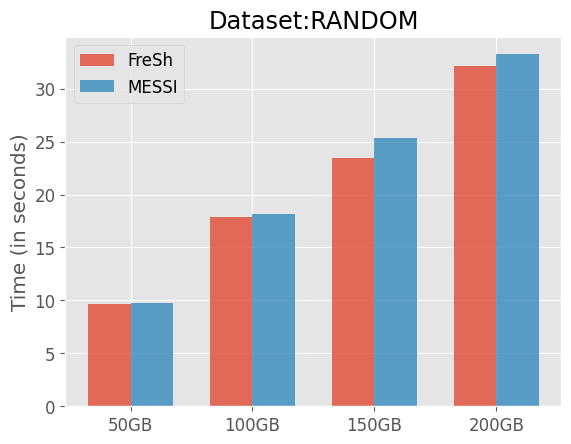
\includegraphics[width=\textwidth]{figures/Experiments/scale-dataset-random-total.png}
        \caption{Total}
        \label{fig:eval:scale-dataset:random:total}
    \end{subfigure}    
    \begin{subfigure}{0.45\textwidth}
        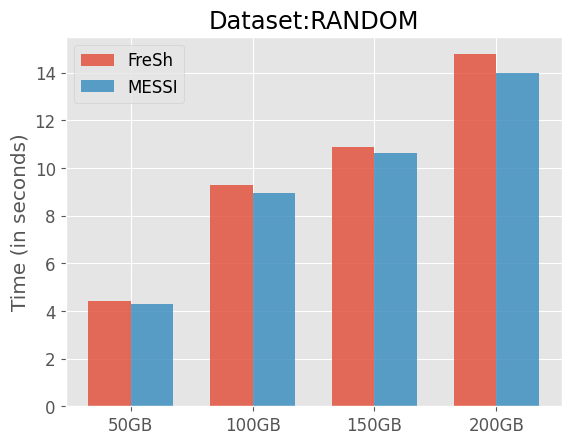
\includegraphics[width=\textwidth]{figures/Experiments/scale-dataset-random-summarization.png}
        \caption{Summarization}
        \label{fig:eval:scale-dataset:random:summarization}
    \end{subfigure}    

    \vspace{0.2cm} % Space between rows

    \begin{subfigure}{0.45\textwidth}
        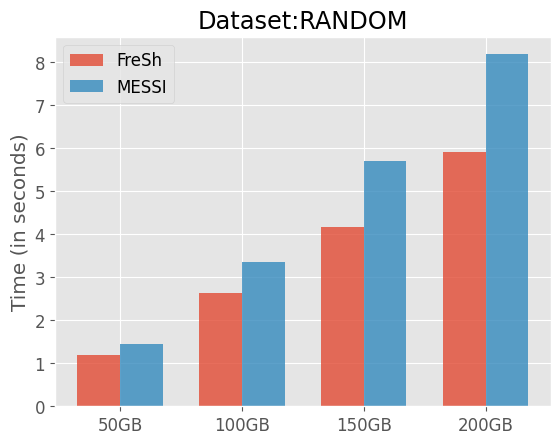
\includegraphics[width=\textwidth]{figures/Experiments/scale-dataset-random-tree.png}
        \caption{Tree index}
        \label{fig:eval:scale-dataset:random:tree-index}
    \end{subfigure}    
    \begin{subfigure}{0.45\textwidth}
        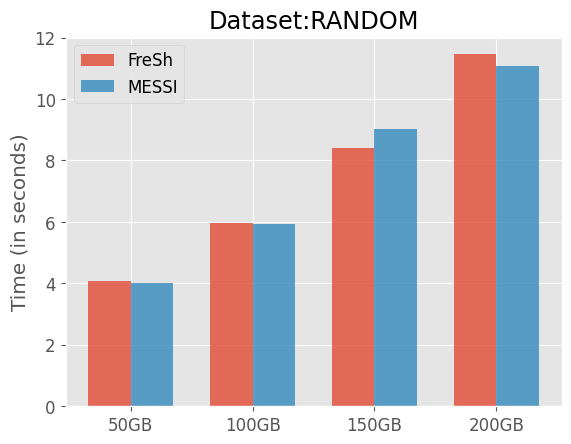
\includegraphics[width=\textwidth]{figures/Experiments/scale-dataset-random-query.png}
        \caption{Query answering}
        \label{fig:eval:scale-dataset:random:query-answering}
    \end{subfigure}                

    \caption{Comparison of \Fresh\ against \MESSI on the Random dataset for 24 threads.}
    \label{fig:eval:scale-dataset:random}
\end{figure}

%%%%%%%%%%%%%%%%%%%%%%%%%%%% REAL DATASETS: DATASET SIZE %%%%%%%%%%%%%%%%%%%%%%%%%%%%%%%%%%%%%%%%%%%%%%%%%%%%%%s

\begin{figure}[htbp]
    \centering
    \begin{subfigure}{0.45\textwidth}
        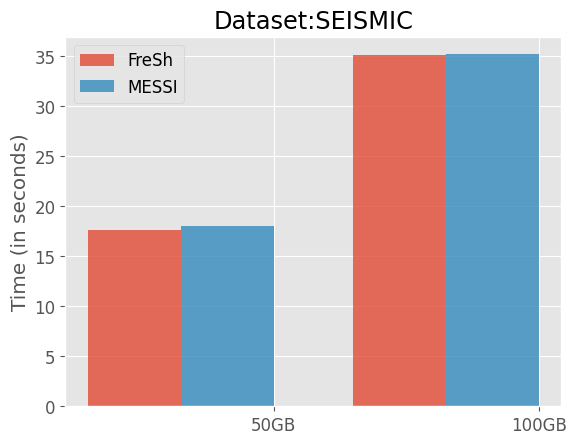
\includegraphics[width=\textwidth]{figures/Experiments/scale-dataset-seismic-total.png}
        \caption{Seismic - Total}
        \label{fig:eval:scale-dataset:seismic:total}
    \end{subfigure}
    \begin{subfigure}{0.45\textwidth}
        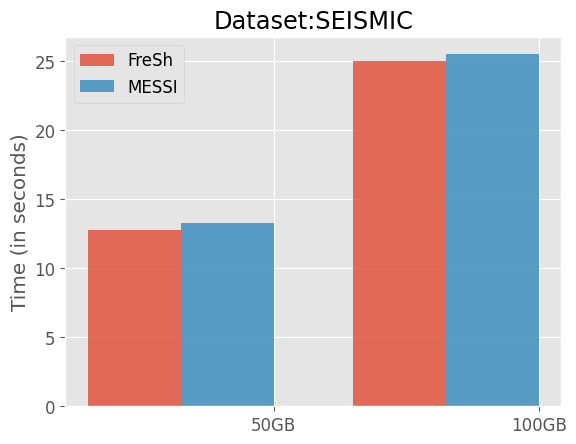
\includegraphics[width=\textwidth]{figures/Experiments/scale-dataset-seismic-query.png}
        \caption{Seismic - Query answering}
        \label{fig:eval:scale-dataset:seismic:QueryAnswering}
    \end{subfigure}        
    \begin{subfigure}{0.45\textwidth}
        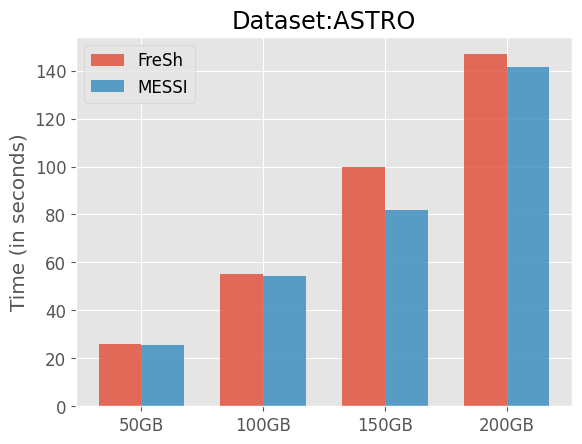
\includegraphics[width=\textwidth]{figures/Experiments/scale-dataset-astro-total.png}
        \caption{Astro - Total}
        \label{fig:eval:scale-dataset:astro:total}
    \end{subfigure}
    \begin{subfigure}{0.45\textwidth}
        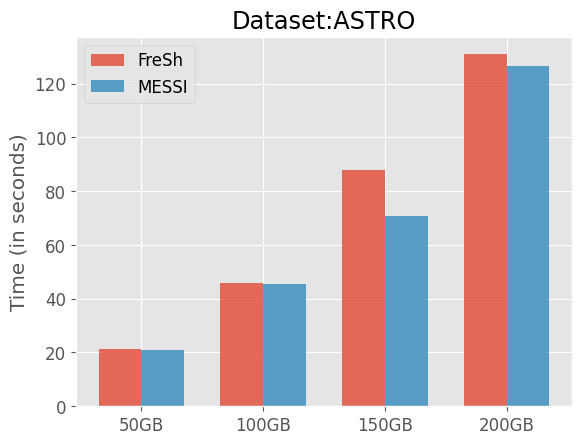
\includegraphics[width=\textwidth]{figures/Experiments/scale-dataset-astro-query.png}
        \caption{Astro - Query answering}
        \label{fig:eval:scale-dataset:astro:QueryAnswering}
    \end{subfigure}    

    \caption{Comparison of \Fresh\ against \MESSI\ on (a) Seismic and (b) Astro datasets for 24 threads.}
    \label{fig:eval:scale-dataset:real}
\end{figure}

%%%%%%%%%%%%%%%%%%%%%%%%%%%%%%%%%%%%%%%%%%%%%%%%%%%%%%%%%%%%%%%%%%%%%%%%%%%%%%%

\begin{figure*}[htbp]
    \centering
    \begin{subfigure}{0.45\textwidth}
        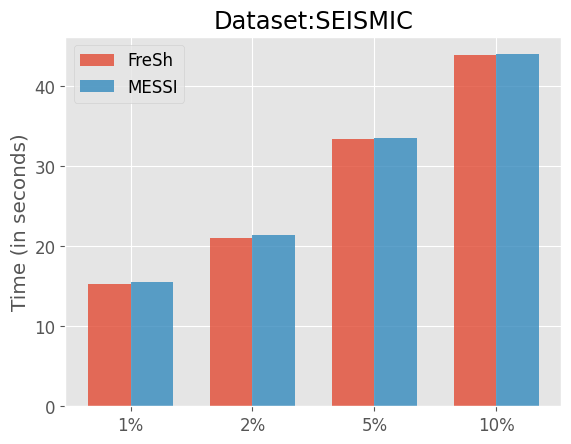
\includegraphics[width=\textwidth]{figures/Experiments/scale-query-difficulty-seismic-total.png}
        \caption{Seismic - Total (Query Difficulty)}
        \label{fig:eval:scale-query-difficulty:seismic:total}
    \end{subfigure}    
    \begin{subfigure}{0.45\textwidth}
        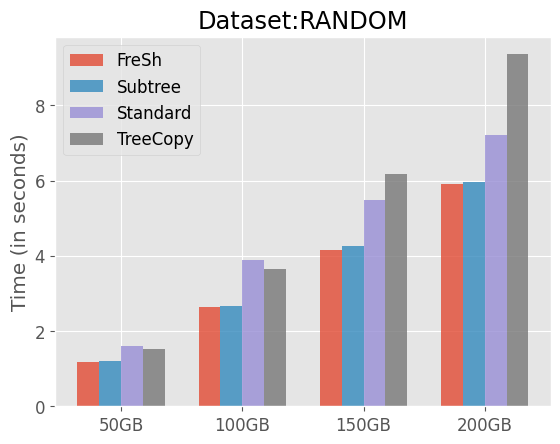
\includegraphics[width=\textwidth]{figures/Experiments/scale-dataset-tree-index-random.png}
        \caption{Tree Index - Random}
        \label{fig:eval:scale-dataset:tree-index:random}
    \end{subfigure}    

    \begin{subfigure}{0.45\textwidth}
        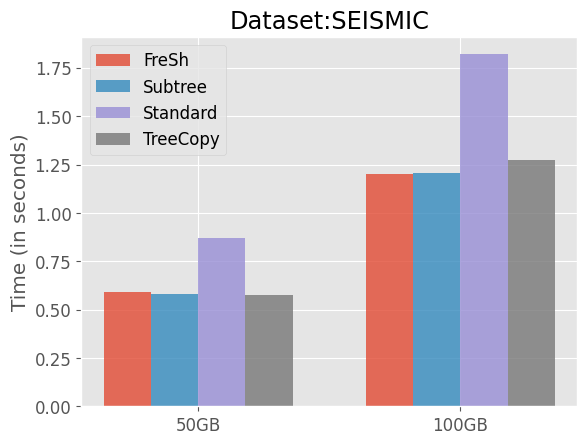
\includegraphics[width=\textwidth]{figures/Experiments/scale-dataset-tree-index-seismic.png}
        \caption{Tree Index - Seismic}
        \label{fig:eval:scale-dataset:tree-index:seismic}
    \end{subfigure}    
    % \begin{subfigure}{0.45\textwidth}
    %     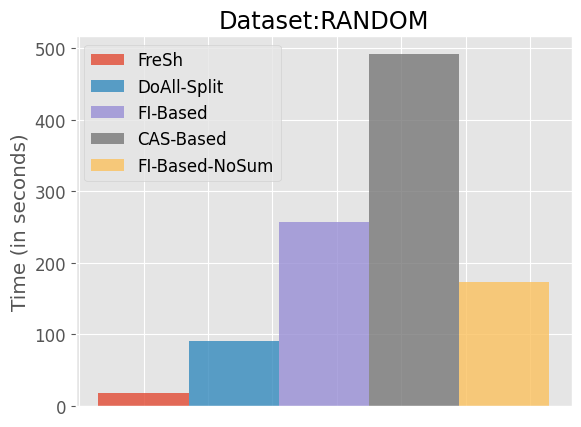
\includegraphics[width=\textwidth]{figures/Experiments/baselines-random-total.png}
    %     \caption{Baseline Comparison - Random}
    %     \label{fig:eval:baselines:random:100GB:total}
    % \end{subfigure}    

    \caption{(a) Comparison of \Fresh\ against \MESSI\ on Seismic 100GB with variable query difficulty, where an increasing percentage of noise is added to the original queries.
    (b)-(c) Comparison of \Fresh\ index creation to other tree implementations.}
    \label{fig:eval:scale-dataset:tree-index}
\end{figure*}


\subsection{ FreSh vs Baselines.}
We compare \Fresh\ against several baseline {\em lock-free} implementations of the 
different stages of an iSAX-based index. 
Our results (Figure~\ref{fig:eval:baselines:random:100GB:total})
shows that \Fresh\ performs better than all these implementations.

\noindent
{\emph{\underline{Summarization Baseline:}}}
For buffer creation, we have experimented with three implementations: \DoAllSplit,
\FI, and \CASBased. All use a single summarization buffer with as many
elements as \RawData.
% 
\DoAllSplit\ splits \RawData\ into as many equaly-sized chunks as the number of threads.  
It stores a {\em done} flag with each data series, which is set after the data series is processed.
Each thread traverses \RawData\ (circularly), starting from the first element of its assigned chunk.
The thread first checks whether the done flag of a data series is set, and processes it only if not. 
%
In \FI, threads use \FAI\ to get assigned data series from \RawData\ to process.  
Each thread $t$ repeatedly performs the following:
It executes a \FAI\ on $O$ to get a position $v$ of RawData,
process the data series stored in this position, and afterwards sets its done flag to \True.
To achieve lock-freedom, \FI\ stores in RawData, a boolean flag (initally false) with each data series. 
This flag, which we call {\em done}, is set to true after the data series has been processed and its iSAX summary 
has been stored in the summarization buffer. 
When a thread figures out that all \RawData\ elements have been assigned,
(i.e., \FAI\ returns a value higher than the number of elements of RawData), 
it re-traverses \RawData\ to identify data series whose done flag is still \False,
and processes them. 
%
\CASBased\ works similarly to \FI, while it uses \CAS\ instructions, instead of \FAI.
%
\Fresh\ performs significantly better than all these implementations
(Fig.~\ref{fig:eval:baselines:random:100GB:total}).


\noindent
{\emph{\underline{Tree Population Baseline:}}}
Each thread is assigned elements of the summarization buffer using \FAI\
and inserts them in the index tree. 
To achieve lock-freedom in traversing the summarization buffer, 
we apply the \DoAllSplit, \FI, and \CASBased\ techniques we describe above.
%
To achieve lock-freedom in accessing the tree, we utilize a flagging technique~\cite{EFR+10},
in addition to our new tree implementation. 
A thread calls a search routine to traverse a path of the tree and reach an appropriate leaf
node $l$. Then, it flags the parent of $l$ using \CAS. If the flagging is successful, the insert
is performed. Then, $l$'s parent is unflagged (using \CAS).
Flagging stores a pointer to an info record in the flagged node.
Other threads may use this info record to help the insert complete. 

We have also experimented with \FINoSum, a lock-free implementation that 
avoids using the summarization buffers and inserts directly iSAX summaries in the index tree, 
by applying the \FI\ technique on \RawData.
%
\Fresh\ performs significantly better than all these implementations
(Figure~\ref{fig:eval:baselines:random:100GB:tree-index}).


\noindent
{\emph{\underline{Pruning Baseline:}}}
All baselines use a single instance of an existing skip-based lock-free priority queue~\cite{LJ13}
to store the candidate data series for refinement.
Threads uses \FAI\ to find the next node to examine in the index tree.
When a thread $t$ discovers that all nodes 
of the tree have been assigned for processing, it re-traverses 
the tree to find nodes that may still  be
unprocessed, and processes them. 
A flag is maintained for each tree node to indicate whether its
processing has been completed. This flag is set when the node is marked as processed. 
During re-traversal, $t$ examines
the flag of each element it visits, and does not process it if 
its flag is set (i.e., if the node is marked as processed).

\noindent
{\emph{\underline{Refinement Baseline:}}}
All threads, repeatedly call DeleteMin
to remove elements from the priority queue, and calculate their real distance computation. 
This simple algorithm is not lock-free as a thread may crash after it has
deleted an element from the queue. In this case, the deleted leaf will not be 
processed. This problem can be easily fixed but that would increase the cost 
of DeleteMin. Experiments show that even the non lock-free simple technique
above is quite costly in comparison to our approach.

Our results show that \Fresh\
performs significantly better than all these implementations,
for query answering time (that includes pruning and refinement, 
Figure~\ref{fig:eval:baselines:random:100GB:query-answering}),.

\begin{figure*}[htbp]
    \centering
    \begin{subfigure}{0.45\textwidth}  
        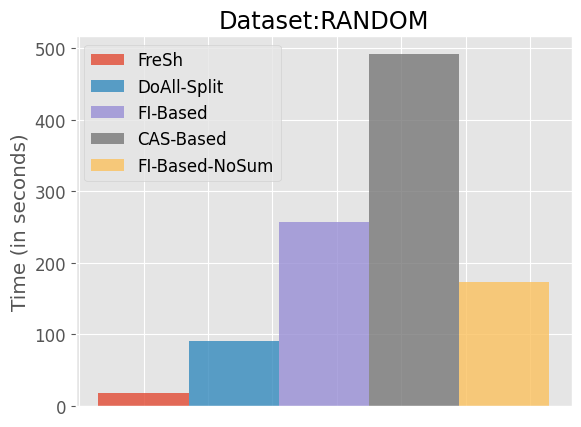
\includegraphics[width=\textwidth]{figures/Experiments/baselines-random-total.png}
        \caption{Total}
        \label{fig:eval:baselines:random:100GB:total}
    \end{subfigure}    
    \begin{subfigure}{0.45\textwidth}  
        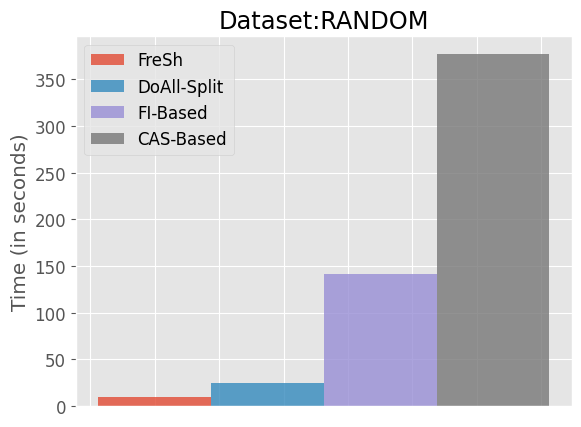
\includegraphics[width=\textwidth]{figures/Experiments/baselines-random-summarization.png}
        \caption{Summarization}
        \label{fig:eval:baselines:random:100GB:summarization}
    \end{subfigure}    

    \begin{subfigure}{0.45\textwidth}  
        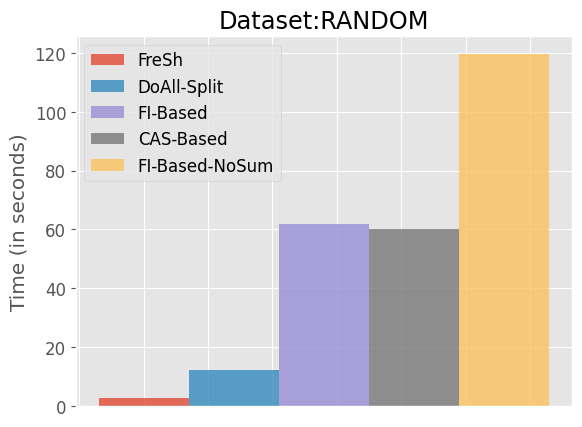
\includegraphics[width=\textwidth]{figures/Experiments/baselines-random-tree.png}
        \caption{Tree index}
        \label{fig:eval:baselines:random:100GB:tree-index}
    \end{subfigure}    
    \begin{subfigure}{0.45\textwidth}  
        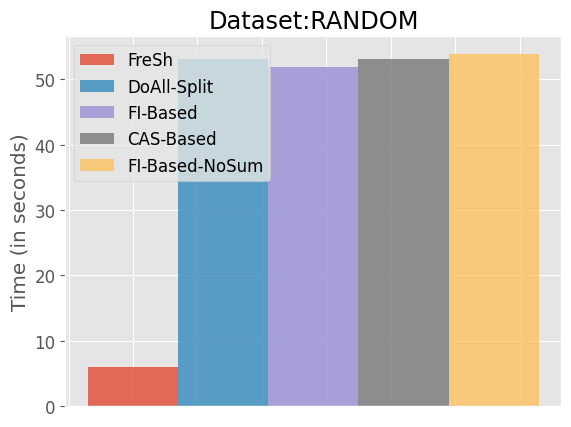
\includegraphics[width=\textwidth]{figures/Experiments/baselines-random-query.png}
        \caption{Query answering}
        \label{fig:eval:baselines:random:100GB:query-answering}
    \end{subfigure}    

    \caption{Comparison of \Fresh\ against baseline implementations on 100GB Random.}
    \label{fig:eval:baselines:random:100GB}
\end{figure*}


%\subsection{Performance breakdown for index creation phase.}

We evaluate the techniques incorporated by \Fresh\ to create its
tree index by comparing it against three modified versions of it. 
Recall that in \Fresh\ each thread populates each of the subtrees it
acquires in expeditive mode, as long as no helper reaches the same leaf of the tree;
when this happens it changes its execution mode to standard. 
So, \Fresh\ allows leaves of the same subtree to be processed in different
modes of execution.

In the first modified version, called \FreshSub, threads start again by populating 
a subtree in expeditive mode, while they change to standard mode as long as a helper 
reaches this subtree (and not when it reaches one of its leaves, as \Fresh\ does); 
so, in \FreshSub\ all the leaves of a subtree are executed in a single mode at each 
point in time. 
In the second modified version, called \FreshSTD, threads populate subtrees using only 
the standard execution mode; i.e., there is no expeditive mode.
In the third modified implementation, called \FreshTreeCopy, a thread $t$ first populates a private
copy of the subtree (i.e. one that is accessible only to $t$) and only after its creation finishes,
$t$ tries to make it the (single) shared version of this subtree (by atomically changing a pointer 
using a \CAS\ instruction); threads help each other by following the same procedure.

Figures~\ref{fig:eval:scale-dataset:tree-index:random}-\ref{fig:eval:scale-dataset:tree-index:seismic}
compare \Fresh\ against the modified versions 
on Random and Seismic with variable dataset sizes and shows that it performs better than them,
in all cases. Interestingly, for Seismic 50GB \Fresh\ performs similarly to \FreshTreeCopy.
Recall that each thread works on its own private copy and, on each subtree, they contend at most once 
on the corresponding \CAS\ object. So, \FreshTreeCopy\ both restricts parallelism and minimizes the 
synchronization cost, which are properties that provide an advantage on Seismic. 


\noindent {\bf Thread Delays.} 
In order to study systems where processes may experience delays (e.g., due to page faults,
time sharing, or long phases of updates),
we came up with a simplistic benchmark, where we simulate delays at random points of a thread's execution. 
We do so by forcing threads to sleep for a specific amount of time, called {\em delay}.
Since \MESSI\ (and \MESSIenh) are lock-based, if a thread crashes, 
the algorithm will never terminate. Thus, we do not perform experiments for this case. 
This is due to the barriers that are utilized in their implementation.
These barriers are necessary for producing correct outcomes and their ignorance even by one thread
could compromise correctness. 
%
Figure~\ref{fig:eval:failure-query:random:failure1} illustrates 
that the delay even of a single thread causes a linear overhead on the performance of \MESSI, 
whereas it hardly has any impact in the performance of \Fresh.
This is so because in \Fresh, helper threads undertake the work to be done by the failed thread,
efficiently compensating the overhead from the failed thread delay.  
%S
Moreover, Figure~\ref{fig:eval:failure-query:random:failure2}
shows that \MESSI\ takes (almost) the full performance hit of delayed threads right from the beginning:
even a single delayed thread blocks 
the execution of all other threads, and hence of the entire algorithm.
\Fresh\ gracefully adapts to the situation of increasing number of delayed threads, 
achieving a speedup. % for Random and Seismic. 
When all-but-one threads fail, \Fresh\ is still faster than \MESSI\ because 
the single non-failing thread helps the others.
%
Note that these synthetic benchmarks are designed to simply illustrate the impact of lock-freedom 
on performance when threads may experience delays (or crash),
and not to capture some realistic setting. % for our studied problem.
Note that \MESSI\ will not terminate execution even if a single thread fails. 
In the case of failures (see Figure~\ref{fig:eval:variable-num-failures}),
\Fresh\ always terminates execution, performing almost identical to \MESSI\ 
with the same number of non-failing threads. This demonstrates that \Fresh adapts
to dynamic thread environments, maintaining high performance levels.


\begin{figure*}[htbp]
    \centering
    \begin{subfigure}{0.45\textwidth}  
        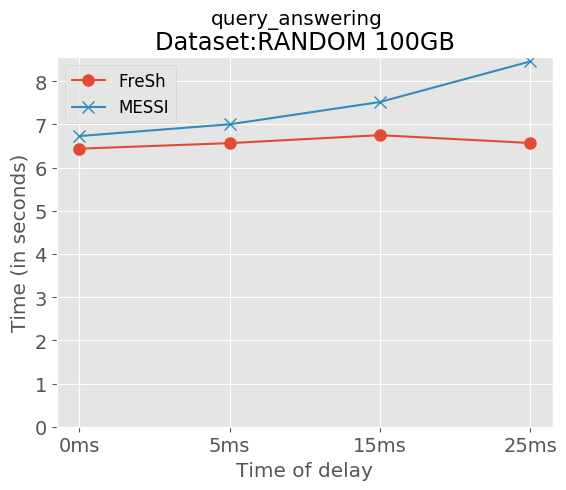
\includegraphics[width=\textwidth]{figures/Experiments/failure-delay-random-query25ms.png}
        \caption{A single thread is delayed.}
        \label{fig:eval:failure-query:random:failure1}
    \end{subfigure}    
    \begin{subfigure}{0.45\textwidth}  
        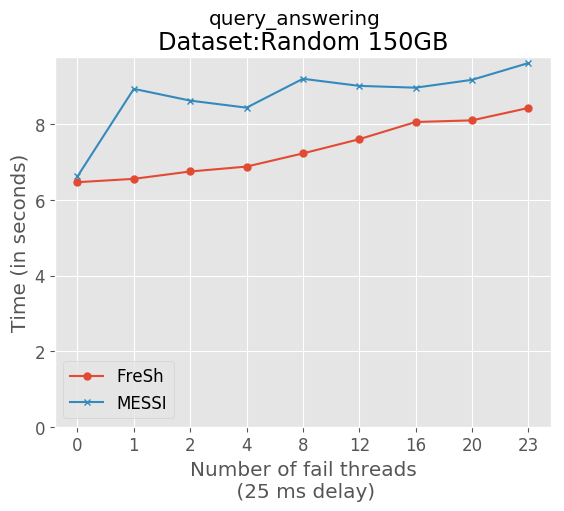
\includegraphics[width=\textwidth]{figures/Experiments/fail-threads-random-query25ms.png}
        \caption{Multiple threads are delayed.}
        \label{fig:eval:failure-query:random:failure2}
    \end{subfigure}    

    \caption{Comparison of \Fresh\ against \MESSI\ when varying delay and number of delayed threads.}
    \label{fig:eval:failure-query:random}
\end{figure*}

\begin{figure*}[htbp]
    \centering
    \begin{subfigure}{0.45\textwidth}  
        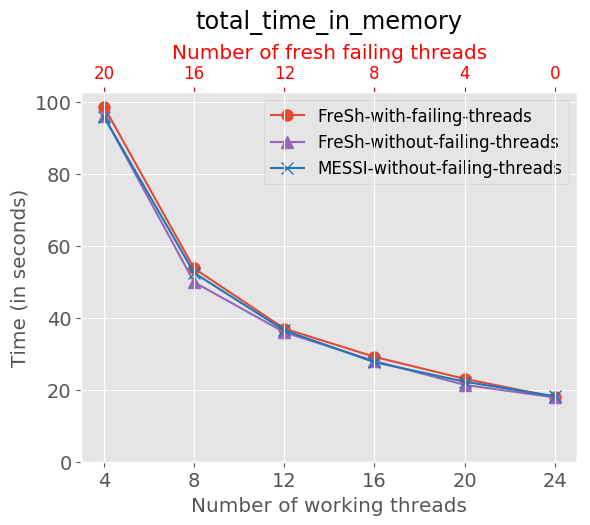
\includegraphics[width=\textwidth]{figures/Experiments/variable-num-failures-total}
        \caption{Total}
        \label{fig:eval:variable-num-failures:total}
    \end{subfigure}    
    \hfill
    \begin{subfigure}{0.45\textwidth}  
        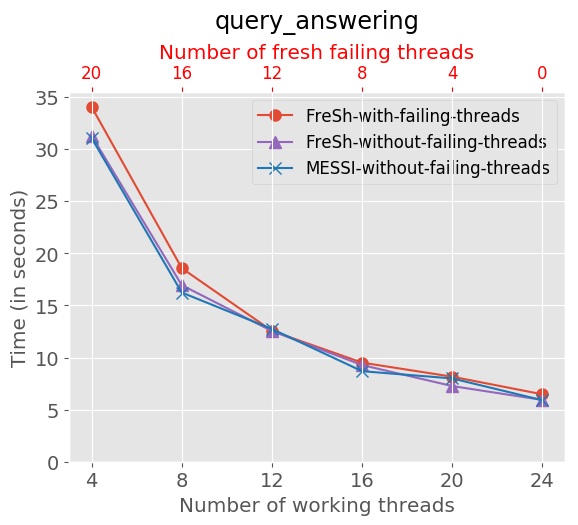
\includegraphics[width=\textwidth]{figures/Experiments/variable-num-failures-query}
        \caption{Query answering}
        \label{fig:eval:variable-num-failures:queries}
    \end{subfigure}    
    \caption{Execution time on Random 100GB, when varying the number of threads that permanently fail 
    (\Fresh with permanent failures in red circles, \Fresh without failures in purple triangles, \MESSI\ without failures in blue crosses).}
    \label{fig:eval:variable-num-failures}
\end{figure*}

\clearpage

\section{Evaluation of Dynamic FreSh}

\noindent{\bf Setup.}
To evaluate DFreSh we used a different machine equipped with 
2 Intel(R) Xeon(R) Gold 5318Y CPU @ 2.10GHz
CPUs with 24 cores each, and 36MB L3 cache. The machine runs
Ubuntu Linux Ubuntu 24.04.1 LTS and has 256GB of RAM. Code is written in 
C and compiled using gcc (Ubuntu 13.2.0-23ubuntu4) 13.2.0 with O2 optimizations.
\noindent{\bf Datasets.} The datasets remain the same.
\noindent{\bf Evaluation Measures.}
We measure (i) the {\em index construction time} , 
(ii) the {\em query answering time} required to answer 50 queries per batch that are not
part of the dataset, 
(iii) we measure the latency of query answering and 
(iv) we provide a comprehend analysis that shows the performace of DFreSh with 
different settings, eg different delays between update batches, (different size of batches). 
Experiments are repeated $5$ times and averages are reported. All the algorithms
return exact results.

\noindent{\bf Latency:}
% 
Query latency is defined as the time between a query's arrival and the start of 
its processing.
% 
As mentioned earlier, queries arrive in batches along with the update batch, meaning 
that all queries in a batch share the same arrival time. The latency of a query is 
defined as the time required to process all pending queries that arrived before it.
%
When the delay is long enough to process all queries in a batch, the latency of the 
$i$-th query can be calculated as the sum of the times required to answer all previous 
queries in the same batch:

\begin{equation}
\text{Latency}(q[i]) = \sum_{j=0}^{i-1} \text{qa}[j]
\end{equation}
% 
where $\text{qa}[j]$ represents the time needed to answer the $j$-th query.
% 
However, if the delay is not sufficient to process all queries within a batch, 
the latency of the $i$-th query is calculated differently. It includes the time 
required to answer the pending queries from previous updates (queries from previous batches) 
and the time for all the queries that arrived before the $i$-th query in the current batch:

\begin{equation}
\text{Latency}(q[i]) = \sum_{j=k}^{n-1} \text{qa}[j] + \sum_{j=0}^{i-1} \text{qa}[j],
\end{equation}
% 
where the first sum accounts for the pending queries from previous updates
and the second sum accounts for the queries from the current batch up to the $i$-th query.
%
For \Fresh\, calculating latency is more complicated because it is a static index, meaning 
query answering begins only after the index construction is complete. The time available 
for answering queries in a given update batch can be expressed as:
\begin{equation}
\text{AvailableQA}(qa[i]) = \text{DELAY} - \text{IC}[i],
\end{equation}
% 
where $\text{AvailableQA}(qa[i])$ represents the available time for answering queries 
in the $i$-th update batch, $\text{DELAY}$ is the delay interval, and $\text{IC}[i]$ 
is the time required to insert the $i$-th batch into the index.
% 
If the delay is sufficient to answer all the queries in time, the latency can be calculated as:

\begin{equation}
\text{Latency}(q[i]) = \text{IC}[i] + \sum_{j=0}^{i-1} \text{qa}[j],
\end{equation}
% 
where $\text{IC}[i]$ represents the time to append the $i$-th batch to the index, and 
$\text{qa}[j]$ is the time required to answer the $j$-th query. If the delay is insufficient, 
unanswered queries from the current batch remain pending and carry over to the next query 
answering period. These pending queries will be processed during the 
$\text{AvailableQA}(qa[i+1])$ interval of the subsequent update batch. 
Thus, the latency can be calculated as:

\begin{equation}
\text{Latency}(q[i]) = \sum_{k=n}^{m} \text{IC}[k] + \sum_{j=0}^{i-1} \text{qa}[j],
\end{equation}
% 
where the $n$-th batch contains the queries in question, and the $m$-th batch represents 
when query $i$ is being answered. If the current batch also includes pending queries from 
previous batches, the latency must also account for the time to answer those queries. 
Thus, the general formula for calculating latency in \Fresh\ is:
% 
\begin{equation}
\text{Latency}(q[i]) = \sum_{k=n}^{m} \text{IC}[k] + \sum_{j=p}^{pq} \text{qa}[j] + \sum_{j=0}^{i-1} \text{qa}[j],
\end{equation}
% 
where $n$ represents the batch that contains the query $i$,-th 
$m$ represents the batch the the $i$-th query is being answered, 
and queries $p$ to $pq$ represents the pending queries from previous baches.


\noindent{\bf Dynamic FreSh vs FreSh.}
We compare the dynamic version of \Fresh, referred to as DFreSh, with \Fresh, 
the current state-of-the-art lock-free in-memory data series index. Our implementation 
includes two versions of DFreSh, each employing a different timestamping algorithm: 
Logical TS and System TS. Additionally, we implemented variations of both that directly 
insert data into the iSAX tree, bypassing the summarization buffers used in 
\Fresh\ during its first phase.
Unlike DFreSh, which supports insertions of batches dynamically, \Fresh\ is a static
system designed to process only a single preloaded dataset. To simulate incoming updates
in \Fresh, the entire dataset must be reloaded with each new update batch appended, requiring 
multiple runs. To ensure a fair comparison, we measure only the time required to 
incorporate the new update batch, isolating the update performance of both systems.

%%%%%%%%%%%%%%%%%%%%%%%%%%%%%%%%%%%%%%%%%%%%%%
\subsection{Evaluation using Random Datatasets}
All experiments performed begin by preloading the index with 10GB of data, called
\textit{initial data} ,followed by processing consecutive batches of $XGB$ until 
whole dataset is processed. For this experimental analysis we have also decided
that each batch is accompanied by 50 new queries. Preloading ensures that even the first 
queries can find answers. We have also desided to add a delay between consecutive batches.
This delay start when a batch arrives and indicates when the next batch is available for
processing.

Figure ~\ref{fig:dfresh-fresh-random} illustrates the overall performance of all 
algorithms when building a 100GB index using random data. Specifically,
figure ~\ref{fig:actual-index-Construction-time} compares the actual index construction times 
of all algorithms, including \Fresh. As expected, the No Buffers version 
perform worse due to reduced cache locality caused by bypassing summarization buffers.
Despite the overhead of managing dynamic updates (e.g such as handling timestamps), 
the buffered versions (Logical and System TS) achieve performance comparable to \Fresh. 
Figure ~\ref{fig:actual-query-answering-time} shows the 
actual query answering time for all algorithms. The buffered versions ouperform No Buffers versions 
because the same index worker operates on a subtree, meaning the cache lines of that worker 
contatin data drom the same subtree leading to improved cache locality. In addition to that
\Fresh\ avoids concurrent reads and writes, reducing cache misses.



The minimum delay, set at 2 seconds (Figure ~\ref{fig:min-delay}), corresponds to the 
time required by the fastest algorithm to answer 50 queries on the smallest index size 
(during the insertion of the first batch). The maximum delay, set at 7 seconds
(Figure ~\ref{fig:max-delay}), allows the slowest algorithm to complete 50 queries on the
largest index size (last batch). In figure~\ref{query-answering-breakdown-random} the bars represent query answering times,
divided into two segments: the light segment indicates concurrent query answering
during index construction, while the dark segment represents solo query answering.
A dark segment indicates insufficient delay, causing some queries to run during
the insertion of other batches.
%
%Once again, the No Buffers versions perform the worst, as cache misses are more costly when not 
%all the data in  a cache line is useful. In contrast, the buffered versions perform better because 
%the same index worker operates on a subtree, meaning the cache lines of that worker 
%contain data from the same subtree, leading to improved cache locality.
Query answering performance is heavily influenced by the delay. Shorter delays result
in poorer performance, as query workers have less time to process the same number
of queries while index construction is ongoing. This results in more pending queries,
increasing computational effort and response times.



%%%%%%%%%%%%%%%%%%%%%%%%% OVERALL PERFORMANCE %%%%%%%%%%%%%%%%%%%%%%%%%%%%%%%%%%%%%%%%%%%%%%%%%%

\begin{figure*}
	\centering
	\begin{subfigure}[c]{0.48\textwidth}
		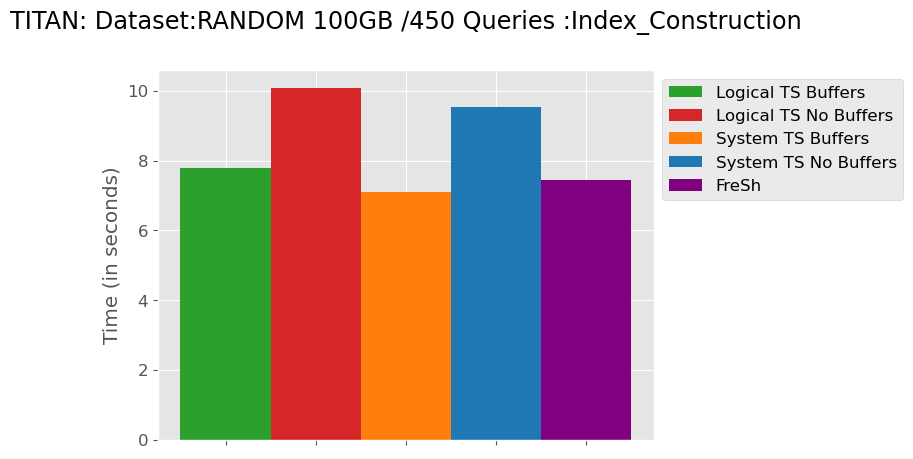
\includegraphics[width=1\textwidth]   {figures/Experiments/Dynamic/Delays/index_construction_all.png}
		\caption{Index Construction Time}
		\label{fig:actual-index-Construction-time}
	\end{subfigure}
	\begin{subfigure}[c]{0.48\textwidth}
		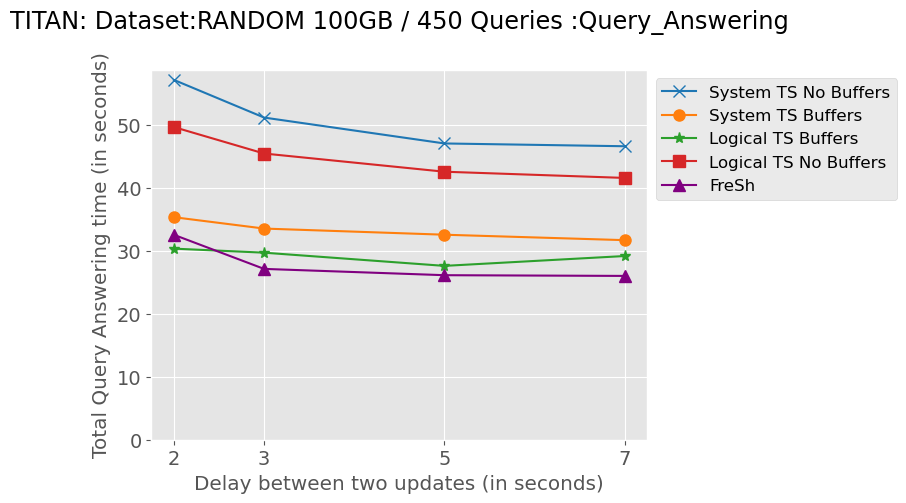
\includegraphics[width=1\textwidth]   {figures/Experiments/Dynamic/Delays/qa_delay_x_axis.png}
		\caption{Query Answering Time}
		\label{fig:actual-query-answering-time}
	\end{subfigure}
	\caption{Dynamic FreSh Benchmarks - Random 100GB/450Q}
	\label{fig:dfresh-fresh-random}
\end{figure*}

%%%%%%%%%%%%%%%%%%%%%%%%%%% Smallest - Largest Delay %%%%%%%%%%%%%%%%%%%%%%%%%%%%%%%%%%%%%%%%%%%%%%%%%%%

\begin{figure*}
	\centering
	\begin{subfigure}[c]{0.48\textwidth}
		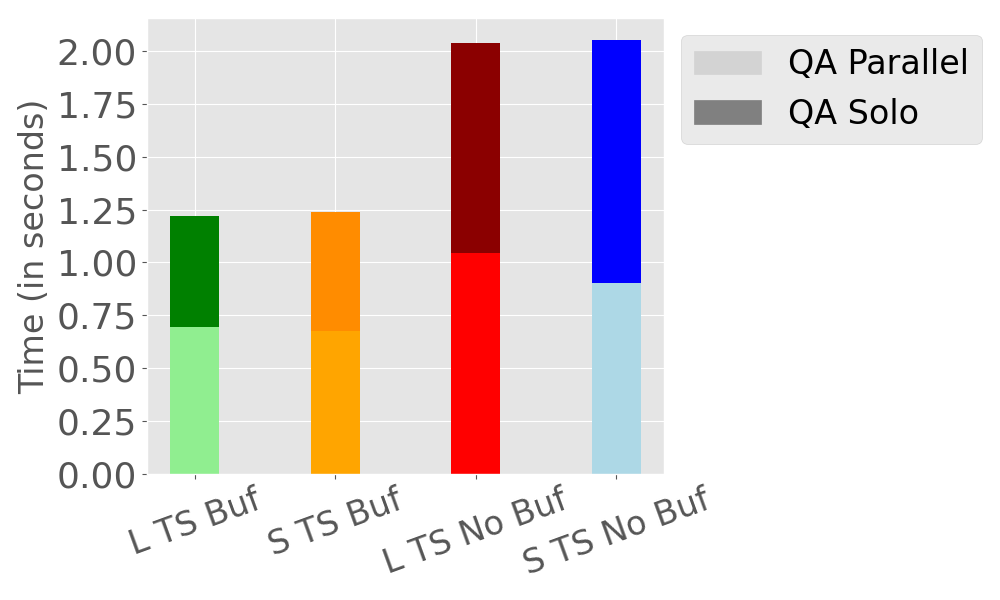
\includegraphics[width=1\textwidth]   {figures/Experiments/Dynamic/Delays/shortest_delay.png}
		\caption{Minimum Delay}
		\label{fig:min-delay}
	\end{subfigure}
	\begin{subfigure}[c]{0.48\textwidth}
		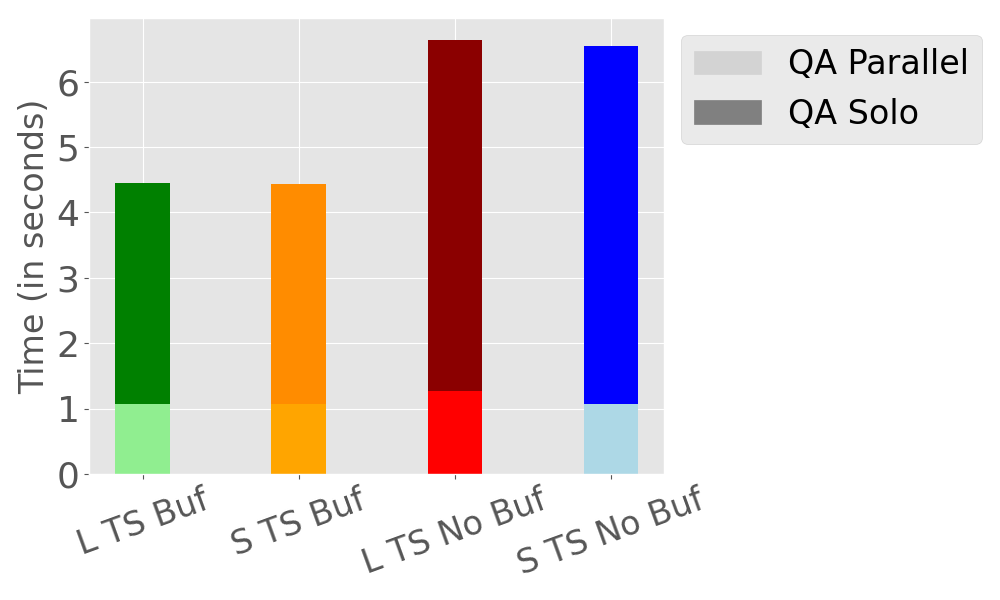
\includegraphics[width=1\textwidth]   {figures/Experiments/Dynamic/Delays/longest_delay.png}
		\caption{Maximum Delay}
		\label{fig:max-delay}
	\end{subfigure}
	\caption{Minimum - Longest Delay}
	\label{fig:min-max-delay}
\end{figure*}

%%%%%%%%%%%%%%%%%%%%%%%%%%%%%%% X AXIS Size %%%%%%%%%%%%%%%%%%%%%%%%%%%%%%%%%%%%%%%%%%%%%%%%%%%%%%%%%%%%%%%
\begin{figure*}
	\centering
	\begin{subfigure}[c]{0.48\textwidth}
		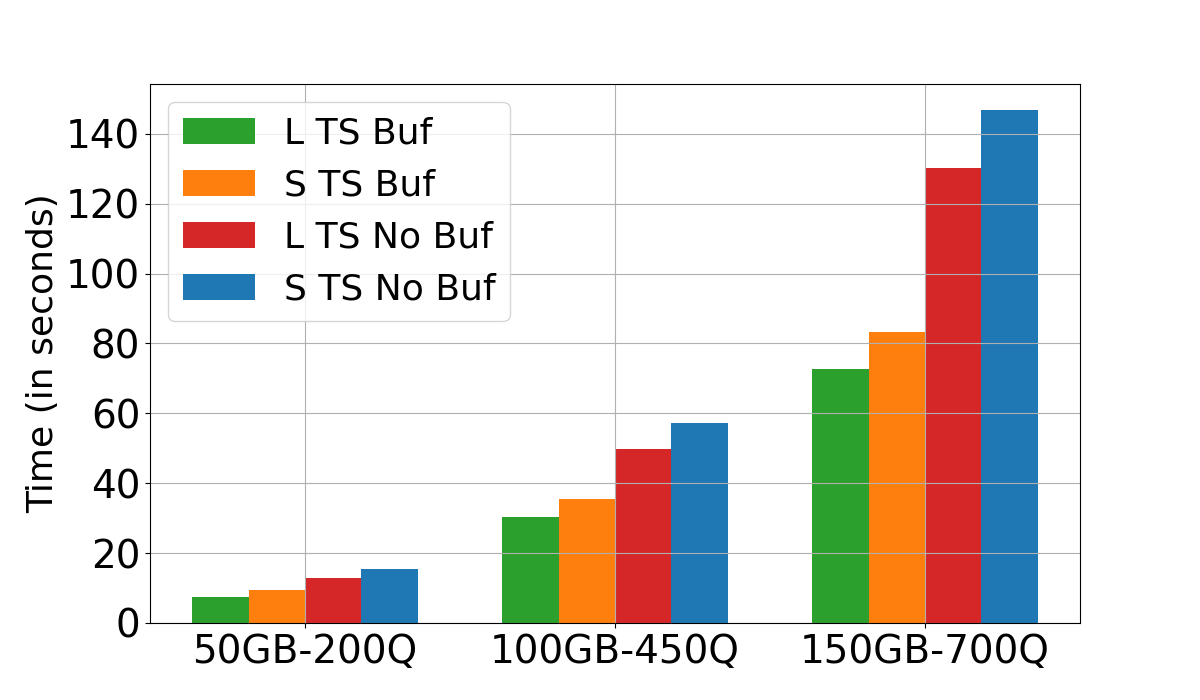
\includegraphics[width=1\textwidth]   {figures/Experiments/Dynamic/xAxis/x_axis_delay[2].png}
		\caption{Query Answering Time Delay 2 sec}
		\label{fig:QA-xAxis-delay-2}
	\end{subfigure}
	\begin{subfigure}[c]{0.48\textwidth}
		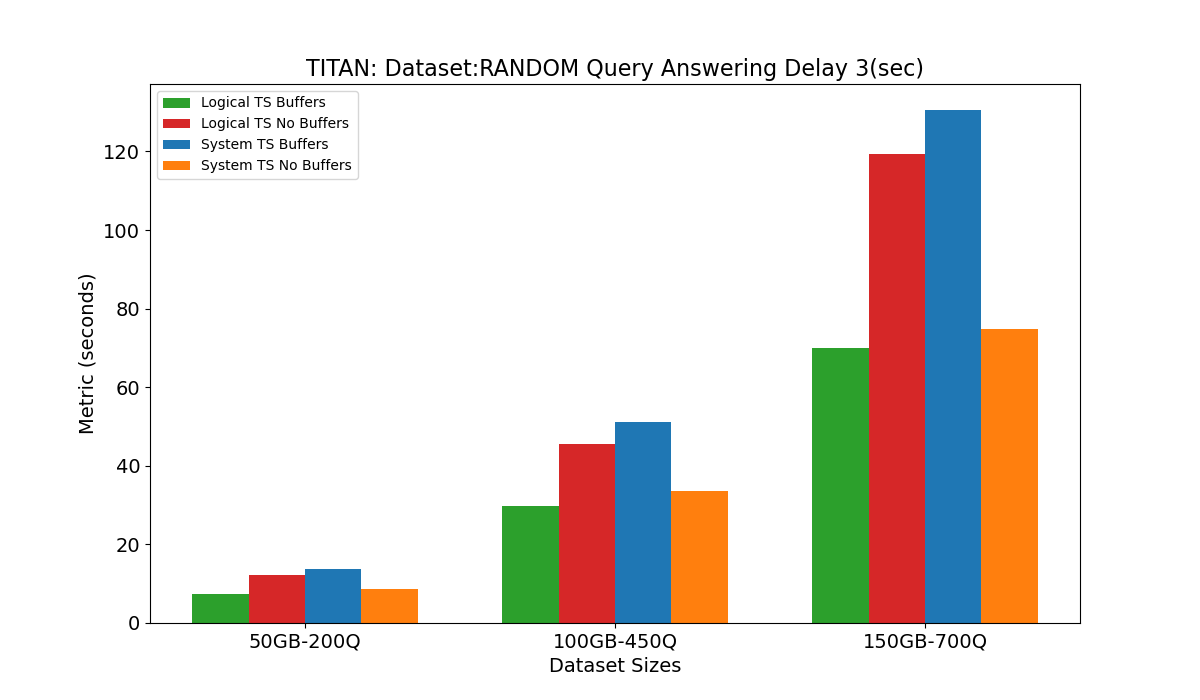
\includegraphics[width=1\textwidth]   {figures/Experiments/Dynamic/xAxis/x_axis_delay[3].png}
		\caption{Query Answering Time Delay 3 sec}
		\label{fig:QA-xAxis-delay-3}
	\end{subfigure}
	\begin{subfigure}[c]{0.48\textwidth}
		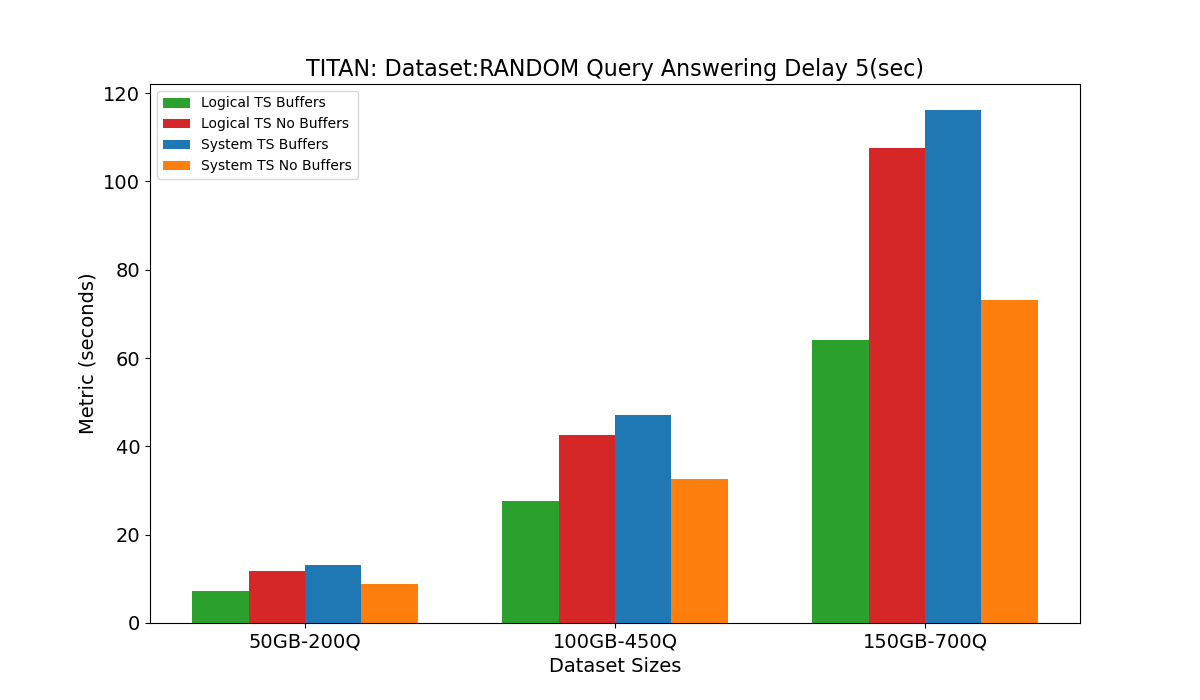
\includegraphics[width=1\textwidth]   {figures/Experiments/Dynamic/xAxis/x_axis_delay[5].png}
		\caption{Query Answering Time Delay 5 sec}
		\label{fig:QA-xAxis-delay-5}
	\end{subfigure}
	\begin{subfigure}[c]{0.48\textwidth}
		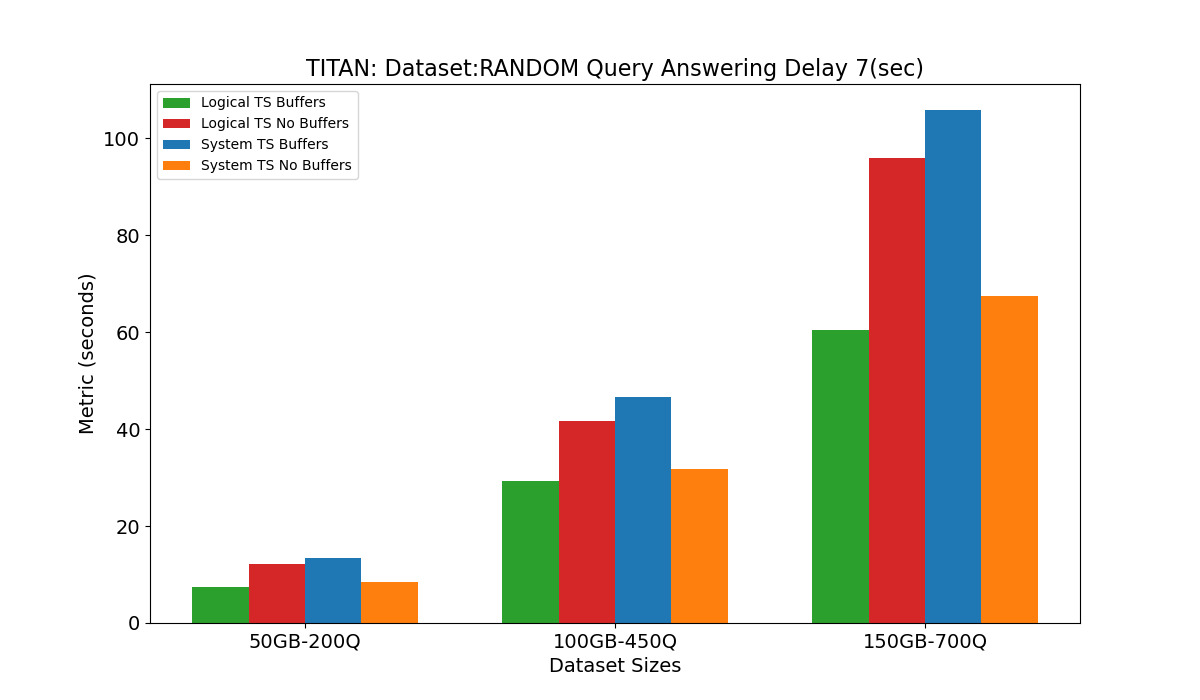
\includegraphics[width=1\textwidth]   {figures/Experiments/Dynamic/xAxis/x_axis_delay[7].png}
		\caption{Query Answering Time Delay 7 sec}
		\label{fig:QA-xAxis-delay-7}
	\end{subfigure}
	\caption{Query Answering Time vs. Index Size}
\end{figure*}


%%%%%%%%%%%%%%%%%%%%%%%%%%%%%% Query Breakdown %%%%%%%%%%%%%%%%%%%%%%%%%%%%%%%%%%%%%%%%%%%%%%%%%%%%%%%%%%%

\begin{figure*}
	\centering
	\begin{subfigure}[c]{0.48\textwidth}
		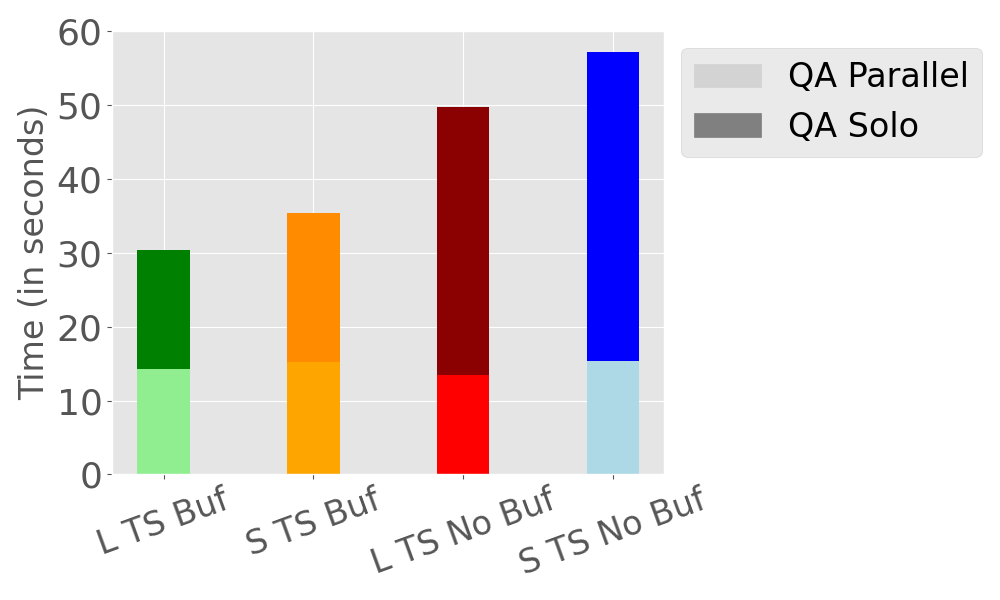
\includegraphics[width=1\textwidth]   {figures/Experiments/Dynamic/Breakdown/dataset_104857600_lockfree_Messi_Results_query_answering_breakdown_10485760_2.png}
		\caption{Delay 2 sec}
		\label{fig:query-answering-breakdown-2}
	\end{subfigure}
	\begin{subfigure}[c]{0.48\textwidth}
		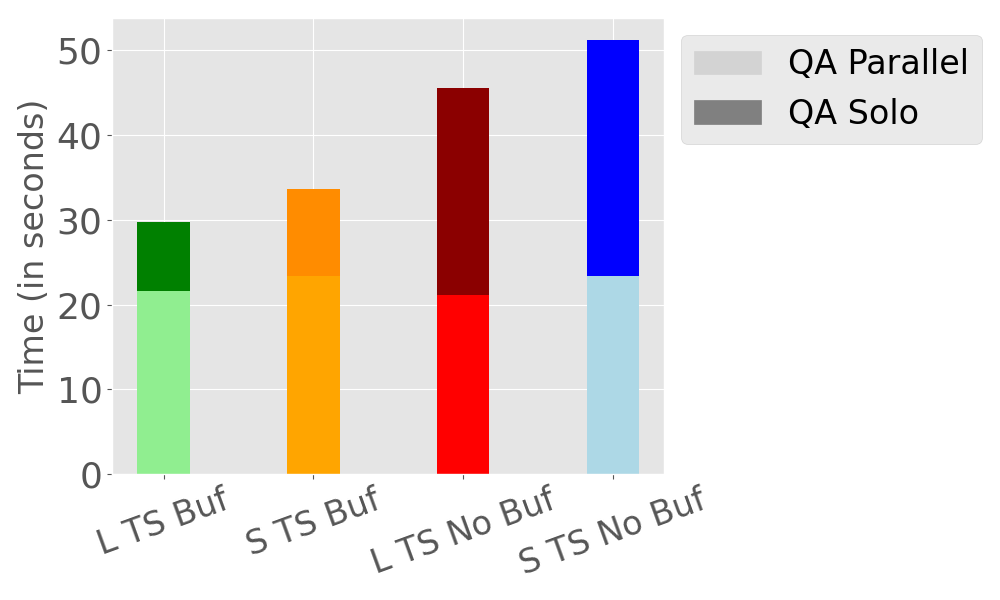
\includegraphics[width=1\textwidth]   {figures/Experiments/Dynamic/Breakdown/dataset_104857600_lockfree_Messi_Results_query_answering_breakdown_10485760_3.png}
		\caption{Delay 3 sec}
		\label{fig:query-answering-breakdown-3}
	\end{subfigure}
	\begin{subfigure}[c]{0.48\textwidth}
		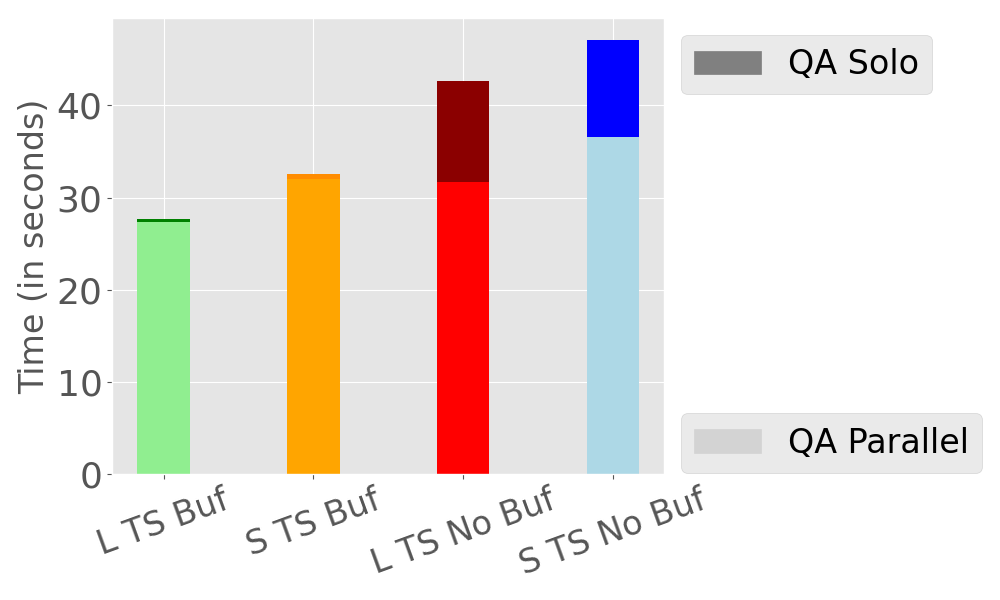
\includegraphics[width=1\textwidth]   {figures/Experiments/Dynamic/Breakdown/dataset_104857600_lockfree_Messi_Results_query_answering_breakdown_10485760_5.png}
		\caption{Delay 5 sec}
		\label{fig:query-answering-breakdown-5}
	\end{subfigure}
	\begin{subfigure}[c]{0.48\textwidth}
		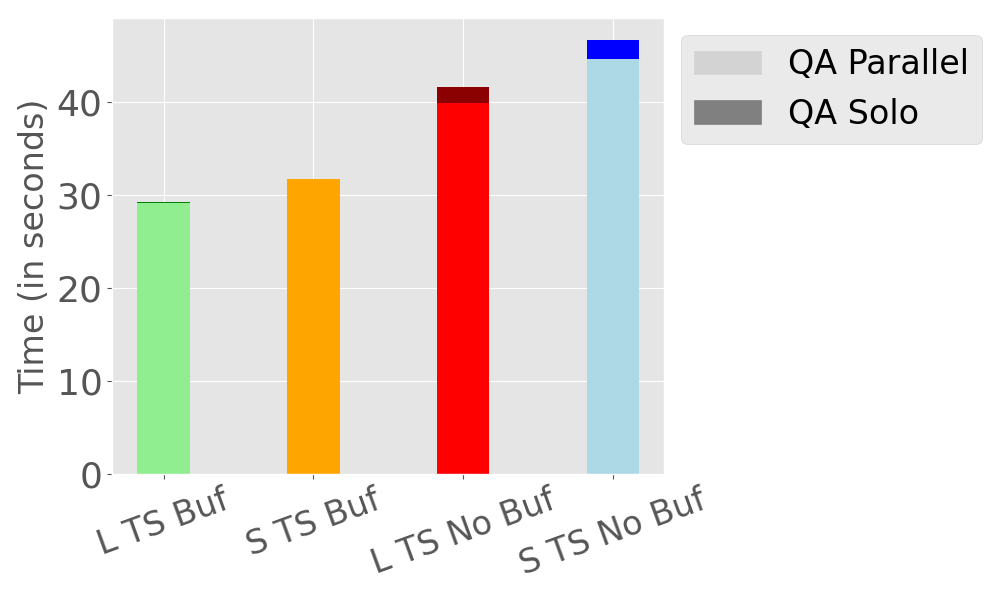
\includegraphics[width=1\textwidth]   {figures/Experiments/Dynamic/Breakdown/dataset_104857600_lockfree_Messi_Results_query_answering_breakdown_10485760_7.png}
		\caption{Delay 7 sec}
		\label{fig:query-answering-breakdown-7}
	\end{subfigure}
	\caption{Query Answering Breakdown - Random 100GB/450Q}
	\label{query-answering-breakdown-random}
\end{figure*}

\clearpage
\subsection{Query Progress}
Figures~\ref{fig:query-progress-delay-2}-\ref{fig:query-progress-delay-7} illustrate
the progress of DFreSh while batches are being inserted. These graphs provide an overview
of the number of queries answered as the index grows, with the x-axis representing the
index size.
%
For example, in Figure~\ref{fig:progress-queries-2-logical}, the first bar shows
that 50 queries were answered between the initial index state and the insertion of
the first batch. This indicates that the implementation of DFreSh using logical timestamps
processes all queries associated with that batch before the next insertion. In contrast,
Figure~\ref{fig:progress-queries-2-system-no-buffers} shows that the implementation
without summarization buffers and using system timestamps answers only 31 out of 50
queries in the same timeframe.
%
These graphs also provide insights into the overall query answering performance, as
summarized in Figure~\ref{fig:actual-query-answering-time}. Notably, as the delay
increases, even the slowest implementations,those without summarization buffers, reduce
the number of queries carried over to subsequent batches. This suggests that with
sufficient delay, even these slower implementations can complete all queries within
the available time.
%%%%% SMALLEST DELAY
\begin{figure*}
	\centering
	\begin{subfigure}[c]{0.45\textwidth}
		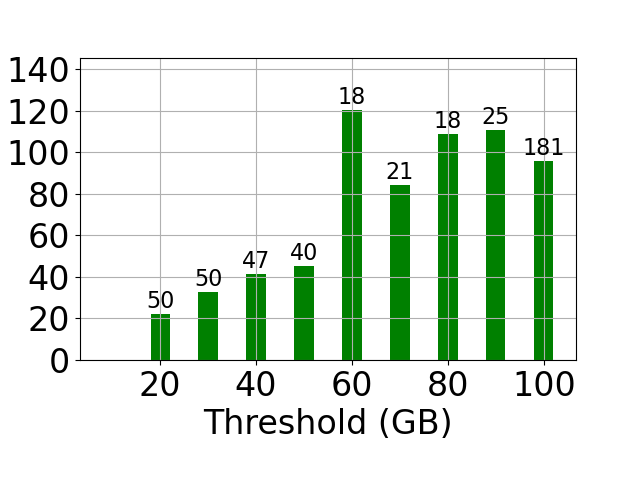
\includegraphics[width=1\textwidth]   {figures/Experiments/Dynamic/Progress/2/average_query_time_per_batch_version_999777015_10485760_10_delay[2].png}
		\caption{Logical TS buffers}
		\label{fig:progress-queries-2-logical}
	\end{subfigure}
	\begin{subfigure}[c]{0.45\textwidth}
		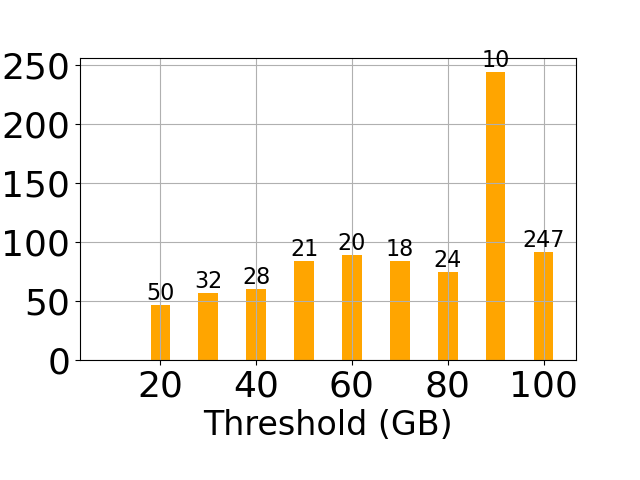
\includegraphics[width=1\textwidth]   {figures/Experiments/Dynamic/Progress/2/average_query_time_per_batch_version_999777018_10485760_10_delay[2].png}
		\caption{System TS buffers}
		\label{fig:progress-queries-2-system}
	\end{subfigure}
	\begin{subfigure}[c]{0.45\textwidth}
		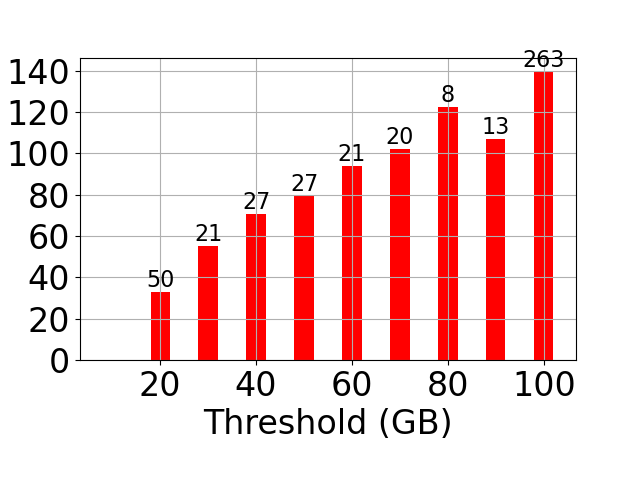
\includegraphics[width=1\textwidth]   {figures/Experiments/Dynamic/Progress/2/average_query_time_per_batch_version_999777016_10485760_10_delay[2].png}
		\caption{Logical TS No buffers}
		\label{fig:progress-queries-2-logical-no-buffers}
	\end{subfigure}
	\begin{subfigure}[c]{0.45\textwidth}
		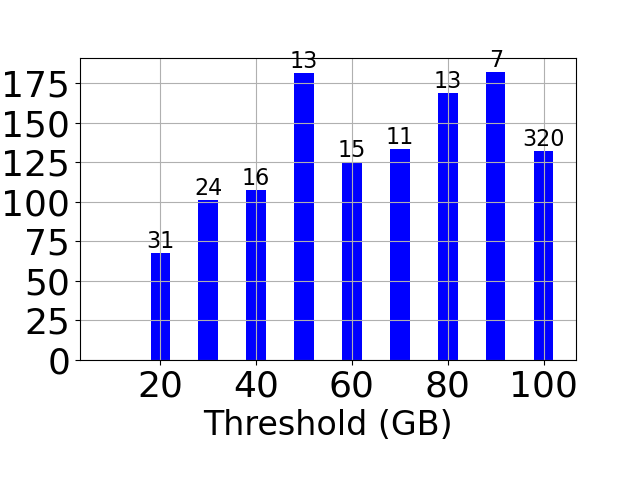
\includegraphics[width=1\textwidth]   {figures/Experiments/Dynamic/Progress/2/average_query_time_per_batch_version_999777017_10485760_10_delay[2].png}
		\caption{System TS No buffers}
		\label{fig:progress-queries-2-system-no-buffers}
	\end{subfigure}
	\caption{Query progress with minimum delay 2 sec.}
	\label{fig:query-progress-delay-2}
\end{figure*}

%%%%%%%%%Intermediate delays 3sec
\begin{figure*}
	\centering
	\begin{subfigure}[c]{0.4\textwidth}
		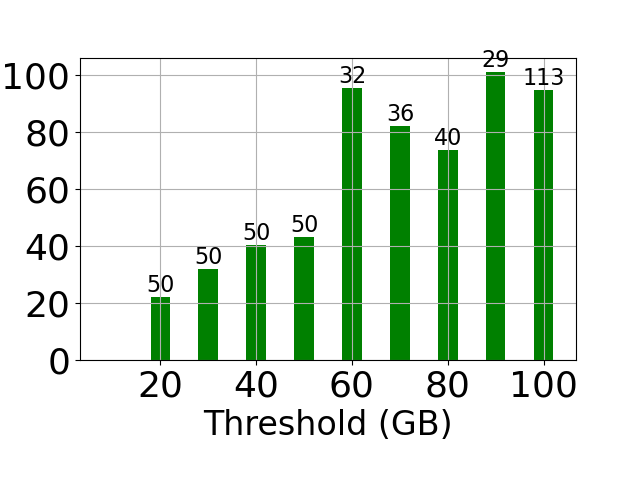
\includegraphics[width=1\textwidth]   {figures/Experiments/Dynamic/Progress/3/average_query_time_per_batch_version_999777015_10485760_10_delay[3].png}
		\caption{Logical TS buffers}
		\label{fig:progress-queries-3-logical}
	\end{subfigure}
	\begin{subfigure}[c]{0.4\textwidth}
		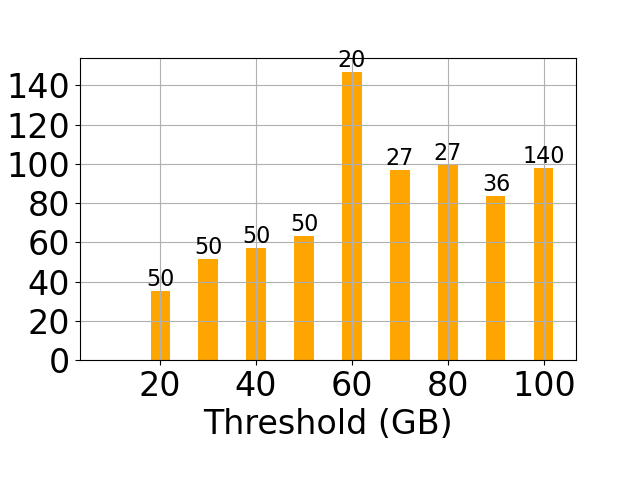
\includegraphics[width=1\textwidth]   {figures/Experiments/Dynamic/Progress/3/average_query_time_per_batch_version_999777018_10485760_10_delay[3].png}
		\caption{System TS buffers}
		\label{fig:progress-queries-3-system}
	\end{subfigure}
	\begin{subfigure}[c]{0.4\textwidth}
		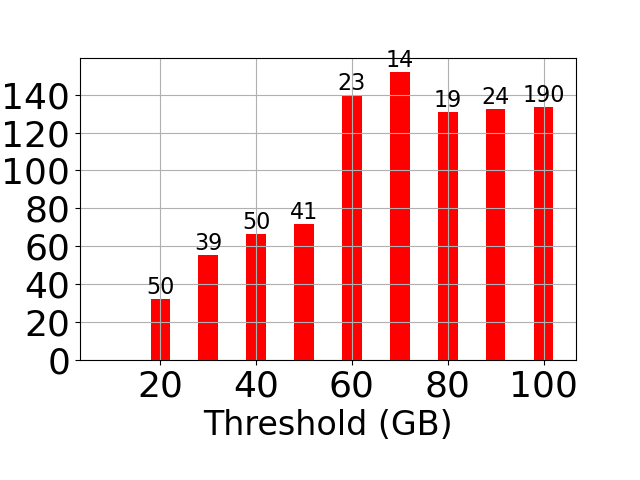
\includegraphics[width=1\textwidth]   {figures/Experiments/Dynamic/Progress/3/average_query_time_per_batch_version_999777016_10485760_10_delay[3].png}
		\caption{Logical TS No buffers}
		\label{fig:progress-queries-3-logical-no-buffers}
	\end{subfigure}
	\begin{subfigure}[c]{0.4\textwidth}
		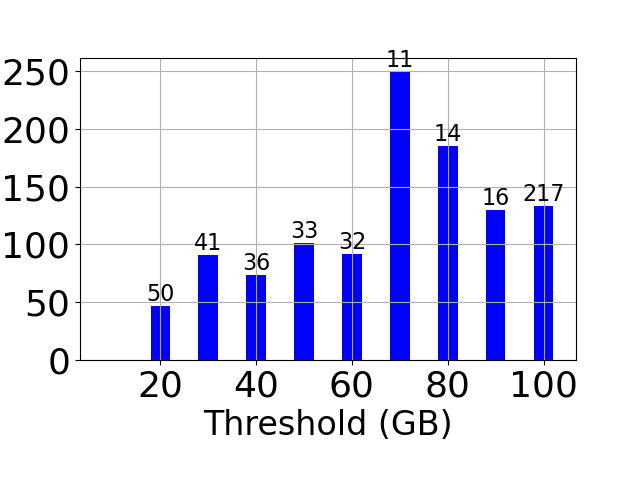
\includegraphics[width=1\textwidth]   {figures/Experiments/Dynamic/Progress/3/average_query_time_per_batch_version_999777017_10485760_10_delay[3].png}
		\caption{System TS No buffers}
		\label{fig:progress-queries-3-system-no-buffers}
	\end{subfigure}
	\caption{Query progress with Intermediate delay 3 sec.}
	\label{fig:query-progress-delay-3}
\end{figure*}


%%%%%%%%%Intermediate delays 5sec
\begin{figure*}
	\centering
	\begin{subfigure}[c]{0.4\textwidth}
		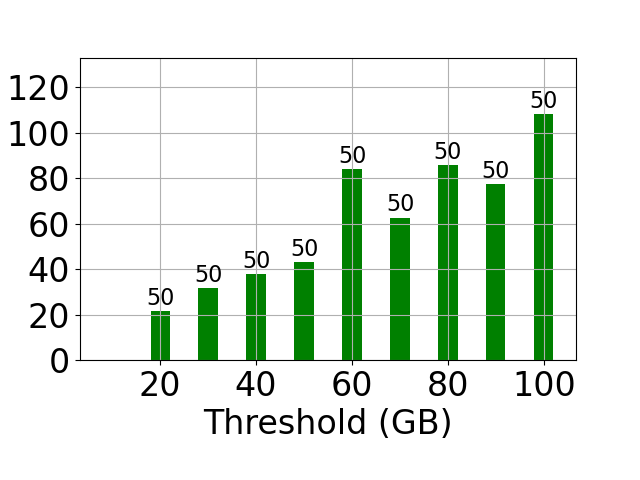
\includegraphics[width=1\textwidth]   {figures/Experiments/Dynamic/Progress/5/average_query_time_per_batch_version_999777015_10485760_10_delay[5].png}
		\caption{Progress of Queries Logical TS buffers}
		\label{fig:progress-queries-5-logical}
	\end{subfigure}
	\begin{subfigure}[c]{0.4\textwidth}
		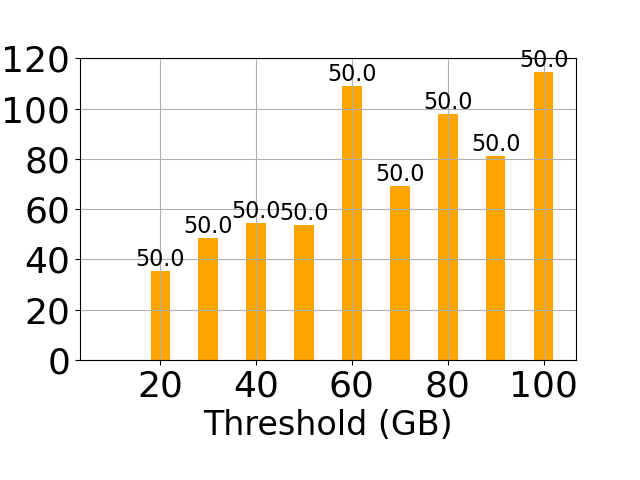
\includegraphics[width=1\textwidth]   {figures/Experiments/Dynamic/Progress/5/average_query_time_per_batch_version_999777018_10485760_10_delay[5].png}
		\caption{Progress of Queries System TS buffers}
		\label{fig:progress-queries-5-system}
	\end{subfigure}
	\begin{subfigure}[c]{0.4\textwidth}
		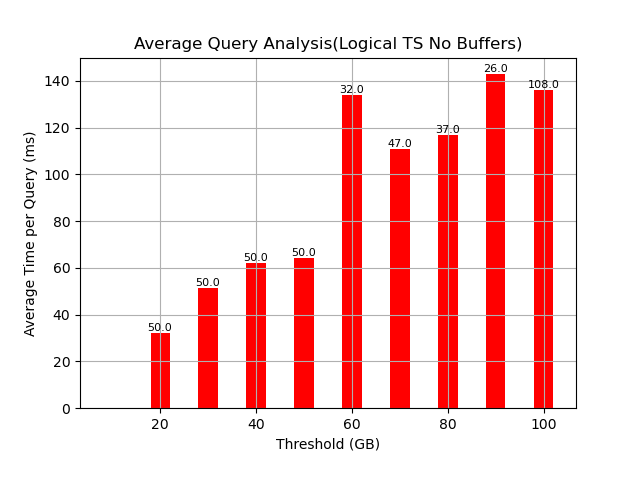
\includegraphics[width=1\textwidth]   {figures/Experiments/Dynamic/Progress/5/average_query_time_per_batch_version_999777016_10485760_10_delay[5].png}
		\caption{Progress of Queries Logical TS No buffers}
		\label{fig:progress-queries-5-logical-no-buffers}
	\end{subfigure}
	\begin{subfigure}[c]{0.4\textwidth}
		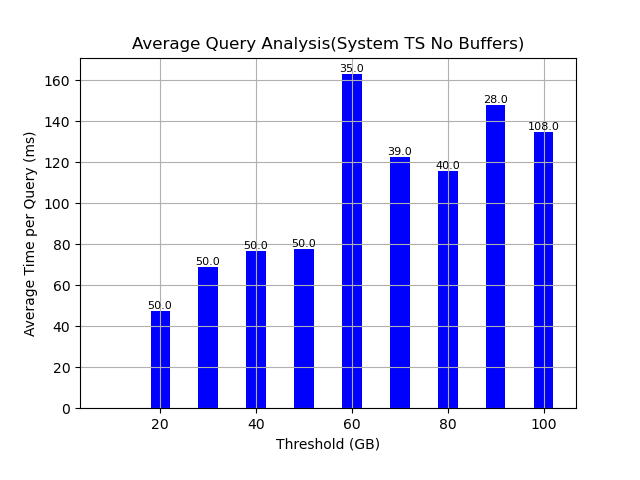
\includegraphics[width=1\textwidth]   {figures/Experiments/Dynamic/Progress/5/average_query_time_per_batch_version_999777017_10485760_10_delay[5].png}
		\caption{Progress of Queries System TS No buffers}
		\label{fig:progress-queries-5-system-no-buffers}
	\end{subfigure}
	\caption{Query progress with Intermediate delay 5 sec.}
	\label{fig:query-progress-delay-5}

\end{figure*}

%%%%% LARGEST DELAY
\begin{figure*}
	\centering
	\begin{subfigure}[c]{0.4\textwidth}
		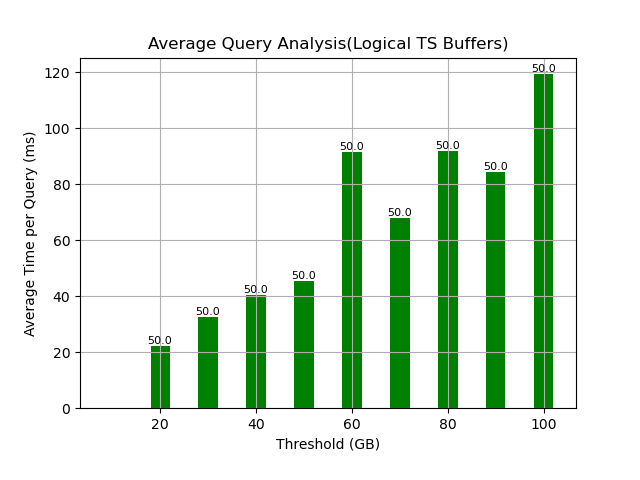
\includegraphics[width=1\textwidth]   {figures/Experiments/Dynamic/Progress/7/average_query_time_per_batch_version_999777015_10485760_10_delay[7].png}
		\caption{Progress of Queries Logical TS buffers}
		\label{fig:progress-queries-7-logical}
	\end{subfigure}
	\begin{subfigure}[c]{0.4\textwidth}
		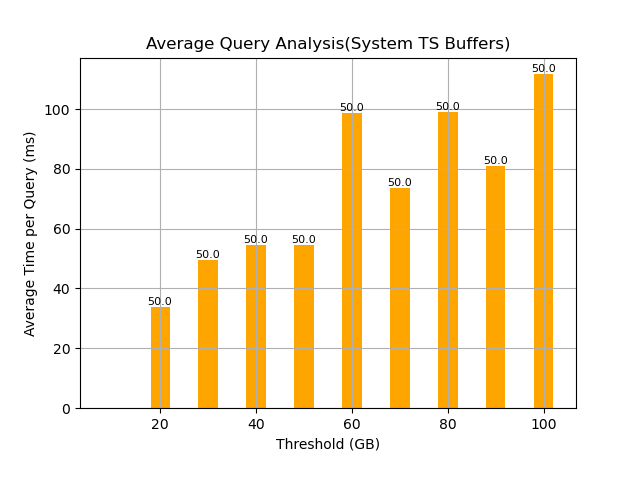
\includegraphics[width=1\textwidth]   {figures/Experiments/Dynamic/Progress/7/average_query_time_per_batch_version_999777018_10485760_10_delay[7].png}
		\caption{Progress of Queries System TS buffers}
		\label{fig:progress-queries-7-system}
	\end{subfigure}
	\begin{subfigure}[c]{0.4\textwidth}
		\includegraphics[width=1\textwidth]   {figures/Experiments/Dynamic/Progress/7/average_query_time_per_batch_version_999777016_10485760_10_delay[7].png}
		\caption{Progress of Queries Logical TS No buffers}
		\label{fig:progress-queries-7-logical-no-buffers}
	\end{subfigure}
	\begin{subfigure}[c]{0.4\textwidth}
		\includegraphics[width=1\textwidth]   {figures/Experiments/Dynamic/Progress/7/average_query_time_per_batch_version_999777017_10485760_10_delay[7].png}
		\caption{Progress of Queries System TS No buffers}
		\label{fig:progress-queries-7-system-no-buffers}
	\end{subfigure}
	\caption{Query progress with largest delay, 7 sec.}
	\label{fig:query-progress-delay-7}
\end{figure*}



\subsection{Latency}

Figure \ref{fig:latency-random} presents the average latency for each query. 

In Figure \ref{fig:latency-random}, System TS Buffers and FreSh exhibit similar latency. 
The key difference between these two implementations, aside from the fact that System TS Buffers 
support dynamic updates, is that System TS Buffers allow concurrent query execution with timestamps 
earlier than the timestamp of the inserting batch. In our implementation, each query receives 
an incrementing timestamp, meaning that the timestamp of query $i+1$ will be larger than that 
of query $i$. As a result, only a small portion of the queries will be fast enough to be answered
before the update batch acquires a timestamp. After this point, queries must wait for the index to 
be completed before they can proceed. In the worst-case scenario for System TS Buffers, queries 
are never fast enough to be answered before the new batch acquires a timestamp, causing it to 
behave similarly to FreSh.

\begin{figure*}
	\centering
	\begin{subfigure}[c]{0.6\textwidth}
		\includegraphics[width=1\textwidth]   {figures/Experiments/Dynamic/Latency/average_latency.png}
		\label{fig:average-latency}
	\end{subfigure}
	\caption{Query Latency - Random 100GB-450Q}
	\label{fig:latency-random}
\end{figure*}

\subsubsection{DFreSh with different batch sizes}

We have also conducted experiments using different batch sizes. In our analysis,
we focus on batch sizes of $5$GB, $10$GB, and $20$GB. Each batch corresponds to
answering $50$ queries. Consequently, for $5$GB batches, we process a total of
$900$ queries over a $100$GB dataset, whereas for $20$GB batches, we process
$250$ queries over a $110$GB dataset, considering that the initial index size
remains $10$GB throughout our experiments.

Figure~\ref{fig:dfresh-fresh-random-different-batches} presents the overall
performance of DFreSh across different batch sizes. The results indicate that the
behavior remains consistent, as batch size does not significantly impact either the
index construction or query answering performance. In particular, the average query
answering time shows only minimal variation across different batch sizes.

\begin{figure*}
	\centering
	\begin{subfigure}[c]{0.45\textwidth}
		\includegraphics[width=1\textwidth]   {figures/Experiments/Dynamic/5GB/7/indexConstruction_7_5GB.png}
		\caption{Real Index Construction Time 5GB Batches}
		\label{fig:actual-index-Construction-time-5GB}
	\end{subfigure}
	\begin{subfigure}[c]{0.45\textwidth}
		\includegraphics[width=1\textwidth]	 {figures/Experiments/Dynamic/5GB/delays_xaxis_5GB.png}
		\caption{Real Query Answering Time 5GB Batches}
		\label{fig:actual-query-answering-time-5GB}
	\end{subfigure}
	\begin{subfigure}[c]{0.45\textwidth}
		\includegraphics[width=1\textwidth]   {figures/Experiments/Dynamic/20GB/7/dataset_115343360_lockfree_Messi_ResultsindexConstruction_7_20GB.png}
		\caption{Real Index Construction Time 20GB Batches}
		\label{fig:actual-index-Construction-time-20GB}
	\end{subfigure}
	\begin{subfigure}[c]{0.45\textwidth}
		\includegraphics[width=1\textwidth]	 {figures/Experiments/Dynamic/20GB/dataset_115343360_lockfree_Messi_Results_query_answering_initial[10485760]_delays_20GB.png}
		\caption{Real Query Answering Time 20GB Batches}
		\label{fig:actual-query-answering-time-20GB}
	\end{subfigure}
	\caption{Dynamic FreSh Benchmarks with different batches}
	\label{fig:dfresh-fresh-random-different-batches}
\end{figure*}


\clearpage
\subsection{Evaluation using Real Datatasets}

This section focuses on experiments conducted using real datasets. Our
experimental analysis of DFreSh requires executing 50 queries per inserted
batch. However, the original dataset contained only 100 queries, which were
insufficient for our experiments. To generate additional queries, we randomly
selected series from the dataset, added Gaussian noise 
($\mu = 0$, $sigma = 0.1$) to each point, and used these modified series 
as queries. Answering queries on real datasets typically requires more time,
as observed in the evaluation of FreSh and previous works, since real queries
tend to be more challenging. The added noise further increases query difficulty,
making the evaluation even more demanding.As a result, the delays used for 
random datasets cannot be applied to real datasets. 
Given that query answering is more computationally intensive than index
construction in this setting, we adjusted the distribution of worker threads
between these tasks. Instead of assigning $36$ workers to index construction
and $12$ to query answering, as in previous experiments, we reversed the
allocation, dedicating $36$ workers to query answering and $12$ to index
construction. This ensures that more computational resources are available
for the more demanding phase of the process.

\noindent{\textbf{Astro Dataset}}  
The initial index size is set to $10$GB, and we use only the first $100$GB
of the dataset. This decision is based on two factors: (1) previous experiments
have shown that dataset size does not affect the average performance of DFreSh,
and (2) the experiment is computationally expensive and time-consuming.


\begin{figure*}
	\centering
	\begin{subfigure}[c]{0.45\textwidth}
		\includegraphics[width=1\textwidth]   {figures/Experiments/Dynamic/ASTRO/index_construction_astro.png}
		\caption{Astro: Real Index Construction Time }
		\label{fig:actual-index-Construction-time-astro}
	\end{subfigure}
	\begin{subfigure}[c]{0.45\textwidth}
		\includegraphics[width=1\textwidth]	 {figures/Experiments/Dynamic/ASTRO/astro_query_answering_xaxis.png}
		\caption{Astro: Real Query Answering Time}
		\label{fig:actual-query-answering-time-astro}
	\end{subfigure}
	\caption{Astro: DFreSh Overall Performance}
	\label{fig:dfresh-performance-astro}
\end{figure*}

Figure~\ref{fig:dfresh-performance-astro} presents the overall performance
of DFreSh. Specifically, Figure~\ref{fig:actual-index-Construction-time-astro}
shows the index construction time, where, as expected, versions utilizing
summarization buffers achieve better performance. We observe that
\textit{System Timestamps} outperform \textit{Logical Timestamps}. 
This is expected, as system timestamps eliminate the need for CAS instructions
during timestamp assignment and reduce concurrency in the iSAX tree between
workers handling different phases due to the waiting protocol we described,
which in turn leads to fewer cache misses. 
Figure~\ref{fig:actual-query-answering-time-astro} illustrates the total query
answering time for processing 450 queries. As expected, summarization buffers
improve performance. Additionally, as the delay increases, different versions
tend to perform better because more queries are processed within each batch.
Consequently, fewer queries are carried over to subsequent batches, reducing
the number of queries that must be answered on an increasingly larger index.

%%%%%%%%%%%%%%%%%%%%%%%%%%%%%%% Query Breakdown %%%%%%%%%%%%%%%%%%%%%%%%%%%%%%
\noindent{\textbf{Query Breakdown}}
%
Figure~\ref{fig:dfresh-query-breakdown-astro} illustrates the distribution of query
answering time in DFreSh. It shows how much of the query processing occurs during the
concurrent execution phase, including the delay times, and how much takes place after
index construction is complete. This distinction is represented by the light and dark
segments of the bars, respectively. Additionally, this figure provides insight into
the difficulty of query answering. The required delay is $10$ times larger than that 
in the Random dataset.

\begin{figure*}
	\centering
	\begin{subfigure}[c]{0.45\textwidth}
		\includegraphics[width=1\textwidth]   {figures/Experiments/Dynamic/ASTRO/breakdown_astro_50.png}
		\caption{Astro: Query Breakdown 50 Delay}
		\label{fig:actual-query-breakdown-50-astro}
	\end{subfigure}
	\begin{subfigure}[c]{0.45\textwidth}
		\includegraphics[width=1\textwidth]	 {figures/Experiments/Dynamic/ASTRO/breakdown_astro_60.png}
		\caption{Astro: Astro: Query Breakdown 60 Delay}
		\label{fig:actual-query-breakdown-60-astro}
	\end{subfigure}
	\begin{subfigure}[c]{0.45\textwidth}
		\includegraphics[width=1\textwidth]	 {figures/Experiments/Dynamic/ASTRO/breakdown_astro_70.png}
		\caption{Astro: Astro: Query Breakdown 70 Delay}
		\label{fig:actual-query-breakdown-70-astro}
	\end{subfigure}
	\caption{Astro: Query Performance Breakdown}
	\label{fig:dfresh-query-breakdown-astro}
\end{figure*}

%%%%%%%%%%%%%%%%%%%%%%%%%%%%%%%% Query Progress %%%%%%%%%%%%%%%%%%%%%%%%%%%%%%%%%%%%%%
\noindent{\textbf{Query Progress}}
%
Figures~\ref{fig:query-progress-50-astro} to~\ref{fig:query-progress-70-astro} show 
the average query answering time as the index size increases. The details of what each
bar represents are explained in the same experiment conducted on the random dataset.
A few observations can be made from these graphs. As expected, as the delay increases,
all versions of DFreSh continue to answer queries in a timely manner. However, in
Figures~\ref{fig:logical-ts-50-astro} to~\ref{fig:system-ts-50-astro}, a different
pattern emerges between the \textit{Logical} and \textit{System} timestamps. Although
\textit{System} timestamps appear fast enough to answer queries promptly in the early
stages, they end up perform worse than \textit{Logical}.
%
From these graphs, we observe that when the index is around half its full capacity,
the average query answering time reaches its peak. This is likely because the queries
being answered during this period are the most difficult or the queries cause contention
and thus cache misses. Since \textit{Logical} timestamps support more concurrency
between workers, they face greater contention, resulting in fewer queries being
answered in that phase. For instance, between the $40$-$60$GB range, the
\textit{System} version answers $89$ queries in total, while the \textit{Logical}
version answers only $80$. However, in the next range ($70$-$80$GB), \textit{Logical}
timestamps manage to close the $9$-query gap, answering queries in a smaller
average time.


\begin{figure*}
	\centering
	\begin{subfigure}[c]{0.45\textwidth}
		\includegraphics[width=1\textwidth]   {figures/Experiments/Dynamic/ASTRO/Batch_processing/50/average_query_time_per_batch_version_999777015_10485760_10_delay[50].png}
		\caption{Astro: Logical TS Buffers}
		\label{fig:logical-ts-50-astro}
	\end{subfigure}
	\begin{subfigure}[c]{0.45\textwidth}
		\includegraphics[width=1\textwidth]	 {figures/Experiments/Dynamic/ASTRO/Batch_processing/50/average_query_time_per_batch_version_999777018_10485760_10_delay[50].png}
		\caption{Astro: System TS Buffers}
		\label{fig:system-ts-50-astro}
	\end{subfigure}
	\begin{subfigure}[c]{0.45\textwidth}
		\includegraphics[width=1\textwidth]	 {figures/Experiments/Dynamic/ASTRO/Batch_processing/50/average_query_time_per_batch_version_999777016_10485760_10_delay[50].png}
		\caption{Astro: Logical TS No Buffers}
		\label{fig:logical-ts-no-50-astro}
	\end{subfigure}
	\begin{subfigure}[c]{0.45\textwidth}
		\includegraphics[width=1\textwidth]	 {figures/Experiments/Dynamic/ASTRO/Batch_processing/50/average_query_time_per_batch_version_999777017_10485760_10_delay[50].png}
		\caption{Astro: System TS No Buffers}
		\label{fig:system-ts-no-50-astro}
	\end{subfigure}
	\caption{Astro: Query Progress 50 delay}
	\label{fig:query-progress-50-astro}
\end{figure*}
%%%%%%%%%%%%%%%%%%%%%%%%%%%%%% Mesaio Delay %%%%%%%%%%%%%%%%%%%%%%%%%%%%%%%%%%%%%%%%%%%%%%%
\begin{figure*}
	\centering
	\begin{subfigure}[c]{0.45\textwidth}
		\includegraphics[width=1\textwidth]   {figures/Experiments/Dynamic/ASTRO/Batch_processing/60/average_query_time_per_batch_version_999777015_10485760_10_delay[60].png}
		\caption{Astro: Logical TS Buffers}
		\label{fig:logical-ts-60-astro}
	\end{subfigure}
	\begin{subfigure}[c]{0.45\textwidth}
		\includegraphics[width=1\textwidth]	 {figures/Experiments/Dynamic/ASTRO/Batch_processing/60/average_query_time_per_batch_version_999777018_10485760_10_delay[60].png}
		\caption{Astro: System TS Buffers}
		\label{fig:system-ts-60-astro}
	\end{subfigure}
	\begin{subfigure}[c]{0.45\textwidth}
		\includegraphics[width=1\textwidth]	 {figures/Experiments/Dynamic/ASTRO/Batch_processing/60/average_query_time_per_batch_version_999777016_10485760_10_delay[60].png}
		\caption{Astro: Logical TS No Buffers}
		\label{fig:logical-ts-no-60-astro}
	\end{subfigure}
	\begin{subfigure}[c]{0.45\textwidth}
		\includegraphics[width=1\textwidth]	 {figures/Experiments/Dynamic/ASTRO/Batch_processing/60/average_query_time_per_batch_version_999777017_10485760_10_delay[60].png}
		\caption{Astro: System TS No Buffers}
		\label{fig:system-ts-no-60-astro}
	\end{subfigure}
	\caption{Astro: Query Progress 60 delay}
	\label{fig:query-progress-60-astro}
\end{figure*}
%%%%%%%%%%%%%%%%%%%%%%%%%% Largest%%%%%%%%%%%%%%%%%%%%%%%%%%%%%%%%%%%%%%%%%%%%%%%%%%%%%%%%
\begin{figure*}
	\centering
	\begin{subfigure}[c]{0.45\textwidth}
		\includegraphics[width=1\textwidth]   {figures/Experiments/Dynamic/ASTRO/Batch_processing/70/average_query_time_per_batch_version_999777015_10485760_10_delay[70].png}
		\caption{Astro: Logical TS Buffers}
		\label{fig:logical-ts-70-astro}
	\end{subfigure}
	\begin{subfigure}[c]{0.45\textwidth}
		\includegraphics[width=1\textwidth]	 {figures/Experiments/Dynamic/ASTRO/Batch_processing/70/average_query_time_per_batch_version_999777018_10485760_10_delay[70].png}
		\caption{Astro: System TS Buffers}
		\label{fig:system-ts-70-astro}
	\end{subfigure}
	\begin{subfigure}[c]{0.45\textwidth}
		\includegraphics[width=1\textwidth]	 {figures/Experiments/Dynamic/ASTRO/Batch_processing/70/average_query_time_per_batch_version_999777016_10485760_10_delay[70].png}
		\caption{Astro: Logical TS No Buffers}
		\label{fig:logical-ts-no-70-astro}
	\end{subfigure}
	\begin{subfigure}[c]{0.45\textwidth}
		\includegraphics[width=1\textwidth]	 {figures/Experiments/Dynamic/ASTRO/Batch_processing/70/average_query_time_per_batch_version_999777017_10485760_10_delay[70].png}
		\caption{Astro: System TS No Buffers}
		\label{fig:system-ts-no-70-astro}
	\end{subfigure}
	\caption{Astro: Query Progress 70 delay}
	\label{fig:query-progress-70-astro}
\end{figure*}

%%%%%%%%%%%%%%%%%%%%%%%%%% Latency %%%%%%%%%%%%%%%%%%%%%%%%%%%%%%%%%%%%%%%%%%%%%%%
\noindent{\textbf{Latency}}
%
Figure~\ref{fig:query-latency} shows the average query latency for the
Astro dataset. As expected, the latency increases as query answering
becomes more resource-intensive. The latency is calculated as described
in the previous sections, and the observed pattern aligns with expectations.

\begin{figure*}
	\centering
	\begin{subfigure}[c]{0.45\textwidth}
		\includegraphics[width=1\textwidth]   {figures/Experiments/Dynamic/ASTRO/average_latency_ASTRO.png}
	\end{subfigure}
	\caption{Astro: Query Latency}
	\label{fig:query-latency}
\end{figure*}
%%%%%%%%%%%%%%%%%%%%%%%%%%%%% SEISMIC DATASET %%%%%%%%%%%%%%%%%%%%%%%%%%%%%%%%%%%%%%%%%%%%%%%%%%%%%%%%%%%
\noindent{\textbf{Seismic Dataset}} 

The initial index size is set to $10$GB, and the total size of the
dataset is limited to  $90$GB.
 
\begin{figure*}
	\centering
	\begin{subfigure}[c]{0.45\textwidth}
		\includegraphics[width=1\textwidth]   {figures/Experiments/Dynamic/SEISMIC/index_construction_seismic.png}
		\caption{Seismic: Real Index Construction Time }
		\label{fig:actual-index-Construction-time-seismic}
	\end{subfigure}
	\begin{subfigure}[c]{0.45\textwidth}
		\includegraphics[width=1\textwidth]	 {figures/Experiments/Dynamic/SEISMIC/query_answering_xaxis.png}
		\caption{Seismic: Real Query Answering Time}
		\label{fig:actual-query-answering-time-seismic}
	\end{subfigure}
	\caption{Seismic: DFreSh Overall Performance}
	\label{fig:dfresh-performance-seismic}
\end{figure*}

Figure~\ref{fig:dfresh-performance-seismic} presents the overall performance of DFreSh
on the Seismic dataset. As with the Astro dataset, 
Figure~\ref{fig:actual-index-Construction-time-seismic} shows that versions utilizing 
summarization buffers achieve better index construction performance. Similarly, 
Figure~\ref{fig:actual-query-answering-time-seismic} illustrates the total query
answering time for processing 400 queries, where summarization buffers again lead to
improved efficiency. Based on our analysis, the chosen delays for this dataset are set
to 25, 35, and 50 seconds. The observations made for the \textit{Astro} dataset also 
apply here, highlighting consistent trends across different real-world datasets.

%%%%%%%%%%%%%%%%%%%%%%%%%%%%%%% Query Breakdown %%%%%%%%%%%%%%%%%%%%%%%%%%%%%%
\noindent{\textbf{Query Breakdown}}
%
Figure~\ref{fig:dfresh-query-breakdown-seismic} illustrates the distribution of query 
answering time in DFreSh for the Seismic dataset. As in the Astro dataset, it
distinguishes between queries processed during the concurrent execution phase,
including delay times, and those answered after index construction is complete,
represented by the light and dark segments of the bars, respectively. Once again,
we observe the increased difficulty of query answering in real datasets compared to
synthetic ones, with the required delay being approximately seven times higher.

\begin{figure*}
	\centering
	\begin{subfigure}[c]{0.45\textwidth}
		\includegraphics[width=1\textwidth]   {figures/Experiments/Dynamic/SEISMIC/25/breakdown_seismic_25.png}
		\caption{Seismic: Query Breakdown 25 Delay}
		\label{fig:actual-query-breakdown-25-seismic}
	\end{subfigure}
	\begin{subfigure}[c]{0.45\textwidth}
		\includegraphics[width=1\textwidth]	 {figures/Experiments/Dynamic/SEISMIC/35/breakdown_seismic_35.png}
		\caption{Seismic: Query Breakdown 35 Delay}
		\label{fig:actual-query-breakdown-35-seismic}
	\end{subfigure}
	\begin{subfigure}[c]{0.45\textwidth}
		\includegraphics[width=1\textwidth]	 {figures/Experiments/Dynamic/SEISMIC/50/breakdown_seismic_50.png}
		\caption{Seismic: Query Breakdown 50 Delay}
		\label{fig:actual-query-breakdown-50-seismic}
	\end{subfigure}
	\caption{Seismic: Query Performance Breakdown}
	\label{fig:dfresh-query-breakdown-seismic}
\end{figure*}

% %%%%%%%%%%%%%%%%%%%%%%%%%%%%%%%% Query Progress %%%%%%%%%%%%%%%%%%%%%%%%%%%%%%%%%%%%%%
 \noindent{\textbf{Query Progress}}
%
Figures~\ref{fig:query-progress-25-seismic} to~\ref{fig:query-progress-50-seismic} 
illustrate the average query answering time as the index size grows. The meaning of
each bar remains the same as in the corresponding experiment on the random dataset.
As expected, increasing the delay allows all versions of DFreSh to maintain timely
query answering. Unlike previous cases, this dataset exhibits no unexpected behavior,
with patterns aligning well with our observations from earlier experiments.

\begin{figure*}
	\centering
	\begin{subfigure}[c]{0.45\textwidth}
		\includegraphics[width=1\textwidth]   {figures/Experiments/Dynamic/SEISMIC/batch_answering/25/average_query_time_per_batch_version_999777015_10485760_10_delay[25].png}
		\caption{Seismic: Logical TS Buffers}
		\label{fig:logical-ts-25-seismic}
	\end{subfigure}
	\begin{subfigure}[c]{0.45\textwidth}
		\includegraphics[width=1\textwidth]	 {figures/Experiments/Dynamic/SEISMIC/batch_answering/25/average_query_time_per_batch_version_999777018_10485760_10_delay[25].png}
		\caption{Seismic: System TS Buffers}
		\label{fig:system-ts-25-seismic}
	\end{subfigure}
	\begin{subfigure}[c]{0.45\textwidth}
		\includegraphics[width=1\textwidth]	 {figures/Experiments/Dynamic/SEISMIC/batch_answering/25/average_query_time_per_batch_version_999777016_10485760_10_delay[25].png}
		\caption{Seismic: Logical TS No Buffers}
		\label{fig:logical-ts-no-25-seismic}
	\end{subfigure}
	\begin{subfigure}[c]{0.45\textwidth}
		\includegraphics[width=1\textwidth]	 {figures/Experiments/Dynamic/SEISMIC/batch_answering/25/average_query_time_per_batch_version_999777017_10485760_10_delay[25].png}
		\caption{Seismic: System TS No Buffers}
		\label{fig:system-ts-no-25-seismic}
	\end{subfigure}
	\caption{Seismic: Query Progress 25 delay}
	\label{fig:query-progress-25-seismic}
\end{figure*}
% %%%%%%%%%%%%%%%%%%%%%%%%%%%%%% Mesaio Delay %%%%%%%%%%%%%%%%%%%%%%%%%%%%%%%%%%%%%%%%%%%%%%%
\begin{figure*}
	\centering
	\begin{subfigure}[c]{0.45\textwidth}
		\includegraphics[width=1\textwidth]   {figures/Experiments/Dynamic/SEISMIC/batch_answering/35/average_query_time_per_batch_version_999777015_10485760_10_delay[35].png}
		\caption{Seismic: Logical TS Buffers}
		\label{fig:logical-ts-35-seismic}
	\end{subfigure}
	\begin{subfigure}[c]{0.45\textwidth}
		\includegraphics[width=1\textwidth]	 {figures/Experiments/Dynamic/SEISMIC/batch_answering/35/average_query_time_per_batch_version_999777018_10485760_10_delay[35].png}
		\caption{Seismic: System TS Buffers}
		\label{fig:system-ts-35-seismic}
	\end{subfigure}
	\begin{subfigure}[c]{0.45\textwidth}
		\includegraphics[width=1\textwidth]	 {figures/Experiments/Dynamic/SEISMIC/batch_answering/35/average_query_time_per_batch_version_999777016_10485760_10_delay[35].png}
		\caption{Seismic: Logical TS No Buffers}
		\label{fig:logical-ts-no-35-seismic}
	\end{subfigure}
	\begin{subfigure}[c]{0.45\textwidth}
		\includegraphics[width=1\textwidth]	 {figures/Experiments/Dynamic/SEISMIC/batch_answering/35/average_query_time_per_batch_version_999777017_10485760_10_delay[35].png}
		\caption{Seismic: System TS No Buffers}
		\label{fig:system-ts-no-35-seismic}
	\end{subfigure}
	\caption{Seismic: Query Progress 35 delay}
	\label{fig:query-progress-35-seismic}
\end{figure*}
% %%%%%%%%%%%%%%%%%%%%%%%%%% Largest%%%%%%%%%%%%%%%%%%%%%%%%%%%%%%%%%%%%%%%%%%%%%%%%%%%%%%%%
\begin{figure*}
	\centering
	\begin{subfigure}[c]{0.45\textwidth}
		\includegraphics[width=1\textwidth]   {figures/Experiments/Dynamic/SEISMIC/batch_answering/50/average_query_time_per_batch_version_999777015_10485760_10_delay[50].png}
		\caption{Seismic: Logical TS Buffers}
		\label{fig:logical-ts-50-seismic}
	\end{subfigure}
	\begin{subfigure}[c]{0.45\textwidth}
		\includegraphics[width=1\textwidth]	 {figures/Experiments/Dynamic/SEISMIC/batch_answering/50/average_query_time_per_batch_version_999777018_10485760_10_delay[50].png}
		\caption{Seismic: System TS Buffers}
		\label{fig:system-ts-50-seismic}
	\end{subfigure}
	\begin{subfigure}[c]{0.45\textwidth}
		\includegraphics[width=1\textwidth]	 {figures/Experiments/Dynamic/SEISMIC/batch_answering/50/average_query_time_per_batch_version_999777016_10485760_10_delay[50].png}
		\caption{Seismic: Logical TS No Buffers}
		\label{fig:logical-ts-no-50-seismic}
	\end{subfigure}
	\begin{subfigure}[c]{0.45\textwidth}
		\includegraphics[width=1\textwidth]	 {figures/Experiments/Dynamic/SEISMIC/batch_answering/50/average_query_time_per_batch_version_999777017_10485760_10_delay[50].png}
		\caption{Seismic: System TS No Buffers}
		\label{fig:system-ts-no-50-seismic}
	\end{subfigure}
	\caption{Seismic: Query Progress 50 delay}
	\label{fig:query-progress-50-seismic}
\end{figure*}

%%%%%%%%%%%%%%%%%%%%%%%%%% Latency %%%%%%%%%%%%%%%%%%%%%%%%%%%%%%%%%%%%%%%%%%%%%%%
\noindent{\textbf{Latency}}
%
Figure~\ref{fig:query-latency-seismic} presents the average query latency for the Seismic
dataset. As expected, its latency follows a similar trend to that of the Astro dataset,
given that both are real datasets. The calculation method remains the same, as described in
previous sections, and the observed pattern is consistent with our expectations.

\begin{figure*}
	\centering
	\begin{subfigure}[c]{0.45\textwidth}
		\includegraphics[width=1\textwidth]   {figures/Experiments/Dynamic/SEISMIC/average_latency_SEISMIC.png}
	\end{subfigure}
	\caption{Seismic: Query Latency}
	\label{fig:query-latency-seismic}
\end{figure*}